\documentclass{beamer}

% xcolor and define colors -------------------------
\usepackage{xcolor}

% https://www.viget.com/articles/color-contrast/
\definecolor{purple}{HTML}{5601A4}
\definecolor{navy}{HTML}{0D3D56}
\definecolor{ruby}{HTML}{9a2515}
\definecolor{alice}{HTML}{107895}
\definecolor{daisy}{HTML}{EBC944}
\definecolor{coral}{HTML}{F26D21}
\definecolor{kelly}{HTML}{829356}
\definecolor{cranberry}{HTML}{E64173}
\definecolor{jet}{HTML}{131516}
\definecolor{asher}{HTML}{555F61}
\definecolor{slate}{HTML}{314F4F}

% Mixtape Sessions
\definecolor{picton-blue}{HTML}{00b7ff}
\definecolor{violet-red}{HTML}{ff3881}
\definecolor{sun}{HTML}{ffaf18}
\definecolor{electric-violet}{HTML}{871EFF}

% Main theme colors
\definecolor{accent}{HTML}{00b7ff}
\definecolor{accent2}{HTML}{871EFF}
\definecolor{gray100}{HTML}{f3f4f6}
\definecolor{gray800}{HTML}{1F292D}


% Beamer Options -------------------------------------

% Background
\setbeamercolor{background canvas}{bg = white}

% Change text margins
\setbeamersize{text margin left = 15pt, text margin right = 15pt} 

% \alert
\setbeamercolor{alerted text}{fg = accent2}

% Frame title
\setbeamercolor{frametitle}{bg = white, fg = jet}
\setbeamercolor{framesubtitle}{bg = white, fg = accent}
\setbeamerfont{framesubtitle}{size = \small, shape = \itshape}

% Block
\setbeamercolor{block title}{fg = white, bg = accent2}
\setbeamercolor{block body}{fg = gray800, bg = gray100}

% Title page
\setbeamercolor{title}{fg = gray800}
\setbeamercolor{subtitle}{fg = accent}

%% Custom \maketitle and \titlepage
\setbeamertemplate{title page}
{
    %\begin{centering}
        \vspace{20mm}
        {\Large \usebeamerfont{title}\usebeamercolor[fg]{title}\inserttitle}\\
        {\large \itshape \usebeamerfont{subtitle}\usebeamercolor[fg]{subtitle}\insertsubtitle}\\ \vspace{10mm}
        {\insertauthor}\\
        {\color{asher}\small{\insertdate}}\\
    %\end{centering}
}

% Table of Contents
\setbeamercolor{section in toc}{fg = accent!70!jet}
\setbeamercolor{subsection in toc}{fg = jet}

% Button 
\setbeamercolor{button}{bg = accent}

% Remove navigation symbols
\setbeamertemplate{navigation symbols}{}

% Table and Figure captions
\setbeamercolor{caption}{fg=jet!70!white}
\setbeamercolor{caption name}{fg=jet}
\setbeamerfont{caption name}{shape = \itshape}

% Bullet points

%% Fix left-margins
\settowidth{\leftmargini}{\usebeamertemplate{itemize item}}
\addtolength{\leftmargini}{\labelsep}

%% enumerate item color
\setbeamercolor{enumerate item}{fg = accent}
\setbeamerfont{enumerate item}{size = \small}
\setbeamertemplate{enumerate item}{\insertenumlabel.}

%% itemize
\setbeamercolor{itemize item}{fg = accent!70!white}
\setbeamerfont{itemize item}{size = \small}
\setbeamertemplate{itemize item}[circle]

%% right arrow for subitems
\setbeamercolor{itemize subitem}{fg = accent!60!white}
\setbeamerfont{itemize subitem}{size = \small}
\setbeamertemplate{itemize subitem}{$\rightarrow$}

\setbeamertemplate{itemize subsubitem}[square]
\setbeamercolor{itemize subsubitem}{fg = jet}
\setbeamerfont{itemize subsubitem}{size = \small}







% Links ----------------------------------------------

\usepackage{hyperref}
\hypersetup{
  colorlinks = true,
  linkcolor = accent2,
  filecolor = accent2,
  urlcolor = accent2,
  citecolor = accent2,
}


% Line spacing --------------------------------------
\usepackage{setspace}
\setstretch{1.2}


% \begin{columns} -----------------------------------
\usepackage{multicol}


% Fonts ---------------------------------------------
% Beamer Option to use custom fonts
\usefonttheme{professionalfonts}

% \usepackage[utopia, smallerops, varg]{newtxmath}
% \usepackage{utopia}
\usepackage[sfdefault,light]{roboto}

% Small adjustments to text kerning
\usepackage{microtype}



% Remove annoying over-full box warnings -----------
\vfuzz2pt 
\hfuzz2pt


% Table of Contents with Sections
\setbeamerfont{myTOC}{series=\bfseries, size=\Large}
\AtBeginSection[]{
        \frame{
            \frametitle{Roadmap}
            \tableofcontents[current]   
        }
    }


% Tables -------------------------------------------
% Tables too big
% \begin{adjustbox}{width = 1.2\textwidth, center}
\usepackage{adjustbox}
\usepackage{array}
\usepackage{threeparttable, booktabs, adjustbox}
    
% Fix \input with tables
% \input fails when \\ is at end of external .tex file
\makeatletter
\let\input\@@input
\makeatother

% Tables too narrow
% \begin{tabularx}{\linewidth}{cols}
% col-types: X - center, L - left, R -right
% Relative scale: >{\hsize=.8\hsize}X/L/R
\usepackage{tabularx}
\newcolumntype{L}{>{\raggedright\arraybackslash}X}
\newcolumntype{R}{>{\raggedleft\arraybackslash}X}
\newcolumntype{C}{>{\centering\arraybackslash}X}

% Figures

% \imageframe{img_name} -----------------------------
% from https://github.com/mattjetwell/cousteau
\newcommand{\imageframe}[1]{%
    \begin{frame}[plain]
        \begin{tikzpicture}[remember picture, overlay]
            \node[at = (current page.center), xshift = 0cm] (cover) {%
                \includegraphics[keepaspectratio, width=\paperwidth, height=\paperheight]{#1}
            };
        \end{tikzpicture}
    \end{frame}%
}

% subfigures
\usepackage{subfigure}


% Highlight slide -----------------------------------
% \begin{transitionframe} Text \end{transitionframe}
% from paulgp's beamer tips
\newenvironment{transitionframe}{
    \setbeamercolor{background canvas}{bg=accent!40!black}
    \begin{frame}\color{accent!10!white}\LARGE\centering
}{
    \end{frame}
}


% Table Highlighting --------------------------------
% Create top-left and bottom-right markets in tabular cells with a unique matching id and these commands will outline those cells
\usepackage[beamer,customcolors]{hf-tikz}
\usetikzlibrary{calc}
\usetikzlibrary{fit,shapes.misc}

% To set the hypothesis highlighting boxes red.
\newcommand\marktopleft[1]{%
    \tikz[overlay,remember picture] 
        \node (marker-#1-a) at (0,1.5ex) {};%
}
\newcommand\markbottomright[1]{%
    \tikz[overlay,remember picture] 
        \node (marker-#1-b) at (0,0) {};%
    \tikz[accent!80!jet, ultra thick, overlay, remember picture, inner sep=4pt]
        \node[draw, rectangle, fit=(marker-#1-a.center) (marker-#1-b.center)] {};%
}

\usepackage{breqn} % Breaks lines

\usepackage{amsmath}
\usepackage{mathtools}

\usepackage{pdfpages} % \includepdf

\usepackage{listings} % R code
\usepackage{verbatim} % verbatim

% Video stuff
\usepackage{media9}

% packages for bibs and cites
\usepackage{natbib}
\usepackage{har2nat}
\newcommand{\possessivecite}[1]{\citeauthor{#1}'s \citeyearpar{#1}}
\usepackage{breakcites}
\usepackage{alltt}

% tikz
\usepackage{tikz}
\usepackage{pgfplots}
\usetikzlibrary{calc, positioning, decorations.pathreplacing, arrows.meta, intersections}
\pgfdeclarelayer{bg}
\pgfdeclarelayer{back}
\pgfdeclarelayer{fg}
\pgfsetlayers{bg,main,fg,back}
\usetikzlibrary{shapes,arrows}

% Setup math operators
\DeclareMathOperator{\E}{E} \DeclareMathOperator{\tr}{tr} \DeclareMathOperator{\se}{se} \DeclareMathOperator{\I}{I} \DeclareMathOperator{\sign}{sign} \DeclareMathOperator{\supp}{supp} \DeclareMathOperator{\plim}{plim}
\DeclareMathOperator*{\dlim}{\mathnormal{d}\mkern2mu-lim}
\newcommand\independent{\protect\mathpalette{\protect\independenT}{\perp}}
   \def\independenT#1#2{\mathrel{\rlap{$#1#2$}\mkern2mu{#1#2}}}
\newcommand*\colvec[1]{\begin{pmatrix}#1\end{pmatrix}}

\newcommand{\myurlshort}[2]{\href{#1}{\textcolor{gray}{\textsf{#2}}}}


\begin{document}

\imageframe{./lecture_includes/mixtape_ci_cover.png}


% ---- Content ----


\section{Introduction to course}

\begin{frame}{Welcome to Mixtape Sessions!}

  \begin{itemize}
    \item Mixtape Sessions is an educational platform designed to ``democratize causal inference'' at all levels by helping bridging people with teachers
    \item Causal inference, in my mind, is an \emph{applied} field as much as it is a \emph{technical} field and so learning more about it is to also learn about a range of topics not normally covered in an econometrics course
    \item These include econometric estimation, detailed exposition of research design elements, but also coding practices, handling of data, more detailed dives on specific topics and even advice on publishing and communicating results
  \end{itemize}

\end{frame}

\begin{frame}{Why Mixtape Sessions}

  \begin{itemize}

    \item Scott Cunningham, Professor of Economics, Baylor University (about me)
    \item Not an econometrician; more of a run of the mill typical applied microeconomist
    \item Workshop is about the science but also the art of causal inference (as is the broader Mixtape Sessions platform)

  \end{itemize}

\end{frame}

\begin{frame}{Class goals}

  \begin{enumerate}
    \item \textbf{Confidence}: You will feel like you have a good understanding of design-based causal inference by the end such that it doesn't feel so mysterious or intimidating
    \item \textbf{Comprehension}: You will have learned a lot both conceptually but also in various specifics, particularly with regards to issues around identification and estimation
    \item \textbf{Competency}: you will have had some experience working together implementing these methods using code in Stata and R, syntax, possession of programs, knowledge of packages
  \end{enumerate}

\end{frame}

\begin{frame}{4-day Causal Inference Workshop}

  TODO: UPDATE THESE
  \begin{itemize}
    \item Our workshop together is 5-days, 8am to 5pm CST, with 15 min breaks on the hour and a 1-hour lunch break at noon CST
    \item It will mix exposition, discussion of papers, coding exercises and discussion as best as I can
    \item It's essentially a semester's worth of material
  \end{itemize}

\end{frame}

\begin{frame}{Github repo}

  \begin{itemize}
    \item We will communicate with one another regularly in the Discord channel and I will always be monitoring it
    \item I will be distributing things to you, like code and slides, via the github repo: \url{github.com/Mixtape-Sessions/Causal-Inference-1}
    \item Each lecture will be recorded and then uploaded to Vimeo as a password protected file that you'll have access to into perpetutity
  \end{itemize}

\end{frame}

\begin{frame}{Topics}

  \begin{enumerate}
    \item Foundations: Day 1
    \item Matching: Day 2
    \item IV: Day 3
    \item RDD: Day 4
  \end{enumerate}

\end{frame}

\begin{frame}{What is causality}

  \begin{quote}
    ``Causation is something that makes a difference, and the difference it makes must be a difference from what would have happened without it.'' -- David Lewis (philosopher)
  \end{quote}

  \bigskip
  Key idea $\rightarrow$ counterfactual. Counterfactuals are neither past nor future.  They are alternative histories created by thought experiments but we use them as framing devices to decipher causality in our timeline

  \bigskip

  Causal inference is also fundamentally practically because if we know causality, then we can also know not only the past, but also the future (policy)

\end{frame}

\begin{frame}{Different types of prediction}

  \begin{columns}
    \column{0.48\linewidth}
    \centering
    \textbf{Prediction machines}
    \begin{itemize}
      \item Traditional prediction seeks to detect patterns in data and fit functional relationships between variables with a high degree of accuracy
      \item ``Does this person have heart disease?'', ``How many books will I sell?''
      \item It is not predictions of what effect a choice will have, though
    \end{itemize}
    \column{0.48\linewidth}
    \centering
    \textbf{Causal inference}
    \begin{itemize}
      \item Causal inference is also a type of prediction, but it's a prediction of a \emph{counterfactual} associated with a particular \emph{choice taken}
      \item Causal inference takes that predicted (or imputed) counterfactual and constructs a causal effect that we hope tells us about a future in the event of a similar choice taken
    \end{itemize}
  \end{columns}
\end{frame}


\begin{frame}{Identification problem}
  \centering
  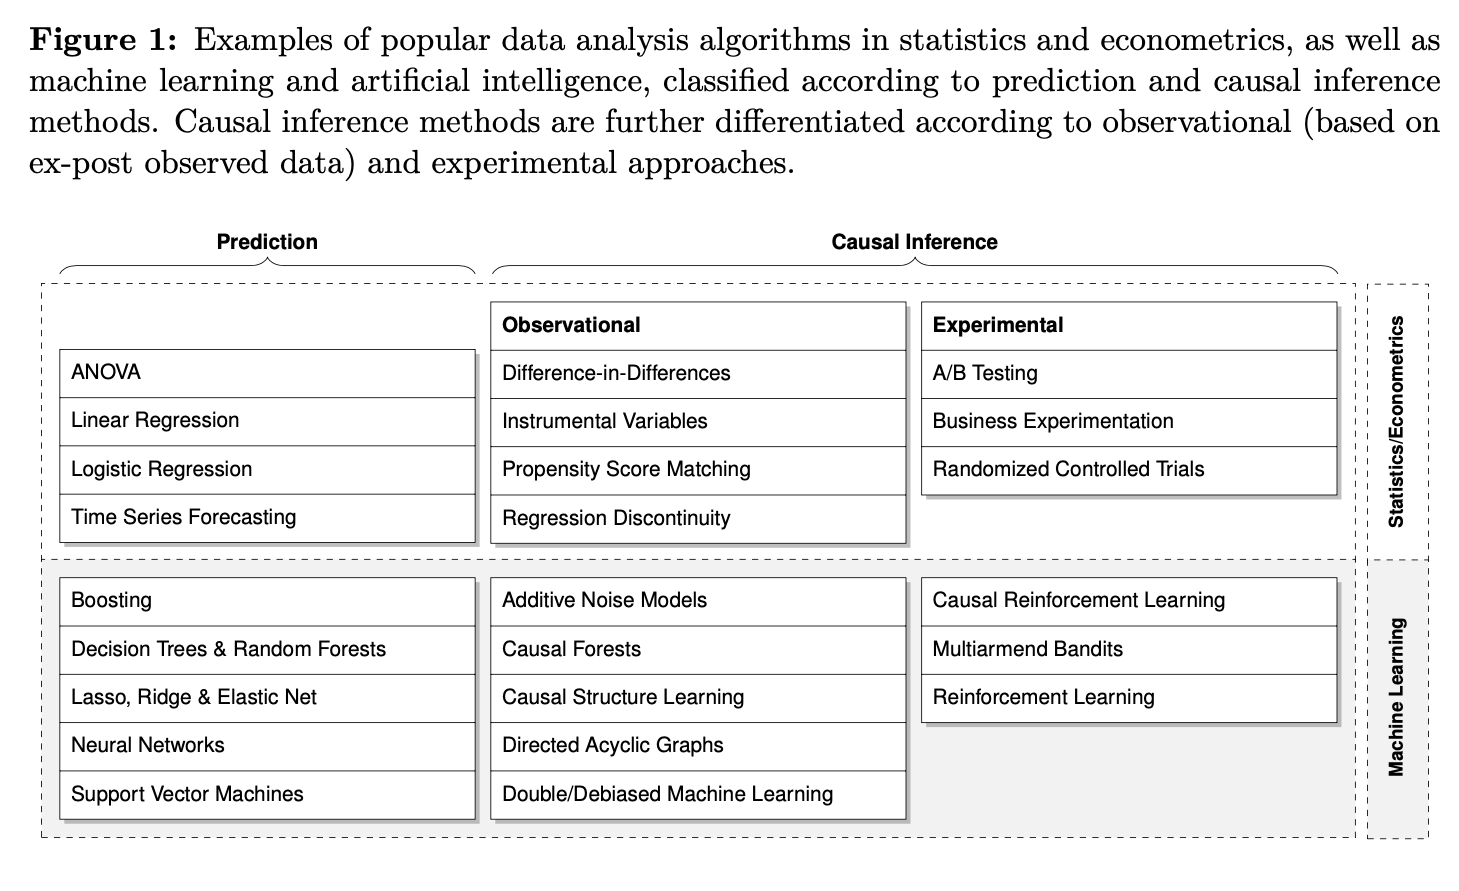
\includegraphics[scale=0.5,height=6.5cm, width=10cm]{./lecture_includes/prediction_causality.png}
\end{frame}



\section{Foundations of causal inference}


\begin{frame}{Some history}

  \begin{itemize}
    \item Causal inference is very old going back millenia
    \item Our class focuses, though, on contemporary causal inference methodologies and practices originating in empirical labor
    \item This is a walk through that history briefly
  \end{itemize}

\end{frame}

\subsection{Princeton Industrial Relations Section}


\begin{frame}{Princeton Industrial Relations Section}

  \begin{itemize}
    \item October 2021's Nobel Prize in economics went to Card, Angrist and Imbens
    \item Princeton's mid 1980s Industrial Relations Section: Orley Ashenfelter, who advises Card, Angrist, LaLonde, hires Krueger, etc.
  \end{itemize}

\end{frame}

\begin{frame}{Princeton and credibility}

  \begin{itemize}
    \item Panel models were not satisfactory for recovering causal effects in Ashenfelter dip situations
    \item Princeton IRS economists focus less on modeling the outcome and more on the treatment variation
    \item LaLonde JMP (AER 1986) as well as Ashenfelter and Card (RESTAT 1985) cast doubt on econometric evaluators, increase demand for explicit randomization
  \end{itemize}

\end{frame}

\begin{frame}{Angrist and Imbens and the 1990s}

  \begin{itemize}
    \item Angrist writes a dissertation using randomized instruments (Vietnam draft), goes to Harvard, overlaps with Imbens for a year, they are mentored by Gary Chamberlain, work with Don Rubin, write their famous LATE paper
    \item Chamberlain recommends potential outcomes framework over a different one that had been used at that time (latent index) and that seems to make the work more generally attractive (like to Rubin)
    \item Let's spend twenty minutes listening to them
  \end{itemize}

\end{frame}

\begin{frame}{Angrist, Imbens and Harvard}


  Josh Angrist on the negative results at the time (10 min)

  \url{https://youtu.be/ApNtXe-JDfA?t=1885}


  \bigskip
  Guido Imbens on the reception of their work (10 min)

  \url{https://youtu.be/cm8V65AS5iU?t=799}

\end{frame}

\subsection{Design versus Model}








\begin{frame}{Causality and the model}

  Empirical labor economics and the economic model (Card speech 2014)

  \bigskip
  \begin{itemize}
    \item \textbf{Model}: Causality exists within the framework of a theory that says ``D causes Y'' (e.g., Heckman)
    \item \textbf{Design}: Causality is design-based and can be discerned with \emph{physical} manipulation of a treatment $D$ (e.g., Rubin, Holland)
  \end{itemize}
\end{frame}


\begin{frame}{Approximating models}

  \begin{enumerate}
    \item[1. ] \textbf{Approximating models}: Consumer demand, labor supply models (e.g., Mincer 1958; 1974)
          \begin{itemize}
            \item Theory implies $y_i=f_i(x_i)$ with restrictions on $f_i$ (e.g., concavity)
            \item Researcher estimates a simpler version $$y_i = \alpha + x_i \beta + \varepsilon_i$$
          \end{itemize}
  \end{enumerate}

\end{frame}

\begin{frame}{Exact models}

  \begin{enumerate}
    \item[2. ] \textbf{Exact models}: Models gives us all causes (``complete DGP'')
          \begin{itemize}
            \item More structural approach to identification, less focused on physical assignment of treatments
            \item Estimate model parameters and distribution of heterogeneity
            \item Functional form, useful for welfare analysis
          \end{itemize}
  \end{enumerate}

\end{frame}

\begin{frame}{Working model}

  \begin{enumerate}
    \item[3. ] \textbf{Working model}: Program evaluation (e.g., Princeton)
          \begin{itemize}
            \item Focus is on physical assignment of treatments (putting it in Fisher tradition on the RCT)
            \item Model formulates questions, intuition, but does not necessarily assist with identification
          \end{itemize}
  \end{enumerate}

  \bigskip

  Empirical labor seems to shift towards more of the ``working model'' approach with exceptions and this is largely connected with an approach that is somewhat agnostic about the underlying model

\end{frame}


\begin{frame}{Topics broaden}

  Dependence on the model vs freed from the model for causal inference increases topics
  \begin{itemize}
    \item \textbf{Design}: Anything goes, ``economics is what economists study'', happiness, fringe stuff (e.g., sex work) (opening up topics)
    \item \textbf{Model}: Neoclassical topics due to needing agreed upon models (limiting topics)
  \end{itemize}

\end{frame}


\begin{frame}{Design's distinctiveness}

  \begin{itemize}
    \item Main idea: focus is on the assignment of units to treatment (e.g., physical randomization, instruments, running variables, propensity score)
    \item Favors deep institutional knowledge and domain knowledge (as opposed to black box style modeling)
    \item Can help answer causal questions when RCTs are difficult to implement (e.g., too expensive, not realistic, not ethical)
    \item Potential outcomes model is really core in all of this
  \end{itemize}

\end{frame}

\subsection{Potential outcomes}

\begin{frame}{Introduction to Counterfactuals}

  \begin{itemize}
    \item Aliens come and orbit earth, see people dying in hospitals and conclude ``doctors are hurting people''
    \item They kill the doctors, unplug patients from machines, throw open the doors -- many patients inexplicably die
    \item \emph{We are the aliens in our research}
  \end{itemize}

\end{frame}

\begin{frame}{\#1: Correlation and causality are different}

  Causal is one unit, correlation is many units
  \begin{itemize}
    \item Causal question: ``If a doctor puts a patient on a ventilator (D), will her covid symptoms (Y) improve?''
    \item Correlation question:  $$\frac{Cov(D,Y)}{\sqrt{Var_D}\sqrt{{Var_Y}}}$$
  \end{itemize}

\end{frame}


\begin{frame}{\#2: Coming first may not mean causality!}

  \begin{itemize}
    \item Every morning the rooster crows and then the sun rises
    \item Did the rooster cause the sun to rise? Or did the sun cause the rooster to crow?
    \item What if cat killed the rooster?
    \item \emph{Post hoc ergo propter hoc}: ``after this, therefore, because of this''
  \end{itemize}

\end{frame}

\begin{frame}[plain]

  \begin{figure}
    \centering
    \includegraphics[scale=0.04]{./lecture_includes/scottboat.jpg}
  \end{figure}

\end{frame}

\begin{frame}{\#3: No correlation does not mean no causality!}

  \begin{itemize}
    \item A sailor sails her sailboat across a lake
    \item Wind blows, and she perfectly counters by turning the rudder
    \item The same aliens observe from space and say ``Look at the way she's moving that rudder back and forth but going in a straight line.  That rudder is broken.'' So they send her a new rudder
    \item They're wrong but why are they wrong? There is, after all, no correlation
    \item Example: Fed and open market operations
  \end{itemize}

\end{frame}

\begin{frame}{History of potential outcomes}

  \begin{itemize}
    \item The conceptual framework for design based causal inference is the \emph{potential outcomes} model which roots causality in counterfactual reasoning
    \item Jerzy Neyman (1923) and Ronald Fisher (1925) linked causal inference to randomized physical experiments
    \item It continues into the present through Donald Rubin in the 1970s and 1980s with Paul Rosenbaum on the propensity score
    \item Continues through Rubin's collaborations with Josh Angrist and Guido Imbens (this year's Nobel Prize winners) on instrumental variables
  \end{itemize}

\end{frame}


\begin{frame}{Potential outcomes notation}

  \begin{itemize}
    \item Let the treatment be a binary variable: $$D_{i,t} =\begin{cases} 1 \text{ if hospitalized at time $t$} \\ 0 \text{ if not hospitalized at time $t$} \end{cases}$$where $i$ indexes an individual observation, such as a person
    \item Potential outcomes: $$Y_{i,t}^j =\begin{cases} 1 \text{ health if hospitalized at time $t$} \\ 0 \text{ health if not hospitalized at time $t$} \end{cases}$$where $j$ indexes a counterfactual state of the world
  \end{itemize}
\end{frame}

\begin{frame}{Moving between worlds}

  \begin{itemize}
    \item I'll drop $t$ subscript, but note -- these are potential outcomes for the same person at the exact same moment in time
    \item A potential outcome $Y^1$ is not the observed outcome $Y$ either conceptually or notationally
    \item Potential outcomes are hypothetical states of the world but observed outcomes are ex post realizations
  \end{itemize}
\end{frame}



\begin{frame}{Important definitions}


  \begin{columns}[t]
    \scriptsize
    \column{.45\textwidth}

    \begin{block}{Definition 1: Individual treatment effect}
      The individual treatment effect,  $\delta_i$, equals $Y_i^1-Y_i^0$
    \end{block}
    \begin{block}{Definition 3: Fundamental problem of causal inference}
      If you need both potential outcomes to know causality with certainty, then since it is impossible to observe both $Y_i^1$ and $Y_i^0$ for the same individual, $\delta_i$, is \emph{unknowable}.
    \end{block}
    \column{.45\textwidth}
    \begin{block}{Definition 2: Switching equation}
      An individual's observed health outcomes, $Y$, is determined by treatment assignment, $D_i$, and corresponding potential outcomes:
      \begin{eqnarray*}
        Y_i& = D_iY^1_i+(1-D_i)Y^0_i& \\
        Y_i& = \begin{cases}
          Y^1_i\text{ if }D_i=1 \\
          Y^0_i\text{ if }D_i=0
        \end{cases}
      \end{eqnarray*}
    \end{block}

  \end{columns}
\end{frame}

\begin{frame}{Missing data problem}

  \begin{itemize}
    \item Causal inference is fundamentally a missing data problem requiring prediction, not of the present or the future, but of a missing past -- sometimes explicitly (nearest neighbor, synthetic control), sometimes implicitly (RDD, IV)
    \item Aggregate parameters based on individual treatment effects are descriptions of causal effects
    \item Fundamental problem of causal inference holds because of the switching equation \emph{even with big data}
  \end{itemize}

\end{frame}


\begin{frame}{Average Treatment Effects}

  \begin{block}{Definition 4: Average treatment effect (ATE)}
    The average treatment effect is the population average of all $i$ individual treatment effects
    \begin{eqnarray*}
      E[\delta_i]&=&E[Y_i^1-Y_i^0]\\
      &=&E[Y^1_i] - E[Y^0_i]
    \end{eqnarray*}
  \end{block}

  \bigskip

  Cannot be calculated because $Y^1_i$ and $Y^0_i$ do not exist \emph{for the same unit i} due to switching equation



\end{frame}



\begin{frame}{Conditional Average Treatment Effects}


  \begin{block}{Definition 5: Average Treatment Effect on the Treated (ATT)}
    The average treatment effect on the treatment group is equal to the average treatment effect conditional on being a treatment group member:
    \begin{eqnarray*}
      E[\delta|D=1]&=&E[Y^1-Y^0|D=1] \nonumber \\
      &=&E[Y^1|D=1]-E[Y^0|D=1]
    \end{eqnarray*}
  \end{block}
  Cannot be calculated because $Y^1_i$ and $Y^0_i$ do not exist \emph{for the same unit i} due to switching equation


\end{frame}

\begin{frame}{Conditional Average Treatment Effects}

  \begin{block}{Definition 6: Average Treatment Effect on the Untreated (ATU)}
    The average treatment effect on the untreated group is equal to the average treatment effect conditional on being untreated:
    \begin{eqnarray*}
      E[\delta|D=0]&=&E[Y^1-Y^0|D=0] \nonumber \\
      &=&E[Y^1|D=0]-E[Y^0|D=0]
    \end{eqnarray*}
  \end{block}
  Cannot be calculated because $Y^1_i$ and $Y^0_i$ do not exist \emph{for the same unit i} due to switching equation

\end{frame}


\begin{frame}{Any collection of treatment effects}

  \begin{itemize}
    \item Notice how in all three of these, all we did was take the defined treatment effect at the individual and aggregate
    \item We will see this again with IV when we introduce the ``local'' average treatment effect
    \item Just keep in mind -- these parameters can be defined, but they cannot be calculated due to the switching equation
  \end{itemize}

\end{frame}

\subsection{Selection bias}

\begin{frame}{Good and bad variation}

  \begin{itemize}
    \item Naive use of statistical models will often find and take advantage of all types of variation for the purpose of prediction
    \item But causal inference is much more cautious because it only uses \emph{some} of the variation
    \item This is better seen with a story and a decomposition
  \end{itemize}

\end{frame}



\begin{frame}{Causality and comparisons}

  \begin{itemize}
    \item Epistemology: what beliefs are warranted and what beliefs are not
    \item Without counterfactuals, we do not \emph{know} treatment effects, but with groups of data we can sometimes obtain \emph{estimates}
    \item We do this by making comparisons of groups treated and not treated
    \item But not all comparisons are equal -- selection bias (e.g., aliens making unwarranted conclusions about causality because of failing to use design)
    \item We will decompose a simple estimator so we can see what \emph{selection bias} is
  \end{itemize}
\end{frame}



\begin{frame}[plain]


  \begin{block}{Definition 7: Simple difference in mean outcomes (SDO)}
    A simple difference in mean outcomes (SDO) can be approximated by the sample averages:\begin{eqnarray*}
      SDO &=& E[Y^1 | D=1] - E[Y^0 | D=0] \\
      &=& E[Y | D=1] - E[Y | D=0]
    \end{eqnarray*}
  \end{block}
  \bigskip
  I tend to use expectation operators $E[ \cdot ]$ but note we are using samples $E_N[ \cdot ]$

\end{frame}

\begin{frame}{SDO}

  \begin{itemize}
    \item Simple difference in mean outcomes is our first estimator
    \item Notice that we switched from potential outcomes to observed outcomes
    \item This means that because the SDO is based on the switching equation, it uses data
    \item So when is the SDO causal and when is it not?
  \end{itemize}

\end{frame}


\begin{frame}{Potentially biased comparisons}

  \begin{block}{Decomposition of the SDO}
    The SDO can be decomposed into the sum of three parts:
    \begin{eqnarray*}
      E[Y^1 | D=1] - E[Y^0 | D=0]&=& ATE\nonumber \\
      &&+ E[Y^0|D=1] - E[Y^0|D=0] \nonumber \\
      && + (1-\pi)(ATT - ATU)
    \end{eqnarray*}
  \end{block}
  Seeing is believing so let's work through this identity!

\end{frame}


\begin{frame}[shrink=20,plain]

  \begin{block}{Use LIE to decompose ATE into the sum of four conditional average expectations}
    \begin{eqnarray*}
      \text{ATE}&=&E[Y^1]-E[Y^0]  \\
      &=& \{\pi E[Y^1 | D=1] + (1-\pi)E[Y^1 | D=0]\}  \\
      & & - \{\pi E[Y^0|D=1] + (1-\pi) E[Y^0 | D=0]\}
    \end{eqnarray*}
  \end{block}


  \begin{block}{Substitute letters for expectations}
    \begin{eqnarray*}
      E[Y^1|D=1] &=& a  \\
      E[Y^1|D=0] &=& b  \\
      E[Y^0|D=1] &=& c  \\
      E[Y^0|D=0] &=& d  \\
      \text{ATE} &=& e
    \end{eqnarray*}
  \end{block}

  \begin{block}{Rewrite ATE}
    \begin{eqnarray*}
      e&=&\{\pi{a} + (1-\pi)b\} - \{\pi{c} + (1-\pi)d\}
    \end{eqnarray*}
  \end{block}

\end{frame}

\begin{frame}[plain]

  \begin{block}{Move SDO terms to LHS}
    \begin{eqnarray*}
      e&=&\{\pi{a} + (1-\pi)b\} - \{\pi{c} + (1-\pi)d\}  \\
      e&=&\pi{a} + b - \pi{b} - \pi{c} - d + \pi{d}  \\
      e&=&\pi{a} + b - \pi{b} - \pi{c} - d + \pi{d} + (\textbf{a} - \textbf{a}) + (\textbf{c} - \textbf{c}) + (\textbf{d} - \textbf{d})  \\
      0&=&e-\pi{a} - b + \pi{b} + \pi{c} + d - \pi{d} - \textbf{a} + \textbf{a} - \textbf{c} + \textbf{c} - \textbf{d} + \textbf{d}  \\
      \textbf{a}-\textbf{d}&=&e-\pi{a} - b + \pi{b} + \pi{c} + d - \pi{d}  + \textbf{a} - \textbf{c} + \textbf{c} - \textbf{d}  \\
      \textbf{a}-\textbf{d}&=&e  + (\textbf{c} - \textbf{d}) + \textbf{a}-\pi{a} - b + \pi{b} - \textbf{c} + \pi{c} + d - \pi{d} \\
      \textbf{a}-\textbf{d}&=&e  + (\textbf{c} - \textbf{d}) + (1-\pi)a -(1-\pi)b + (1-\pi)d - (1-\pi)c  \\
      \textbf{a}-\textbf{d}&=&e  + (\textbf{c} - \textbf{d}) + (1-\pi)(a-c) -(1-\pi)(b-d)
    \end{eqnarray*}
  \end{block}


\end{frame}

\begin{frame}[shrink=20,plain]
  \begin{block}{Rewrite from previous slide}
    \begin{eqnarray*}
      \textbf{a}-\textbf{d}&=&e  + (\textbf{c} - \textbf{d}) + (1-\pi)(a-c) -(1-\pi)(b-d)
    \end{eqnarray*}
  \end{block}

  \begin{block}{Substitute conditional means}
    \begin{eqnarray*}
      E[Y^1|D=1] - E[Y^0|D=0] &=& \text{ATE}  \\
      &&+ (E[Y^0|D=1] - E[Y^0|D=0])  \\
      && + (1-\pi)(\{E[Y^1|D=1] - \alert{E[Y^0|D=1]}\}  \\
      && - (1-\pi)\{\alert{E[Y^1|D=0]} - E[Y^0|D=0]\}) \\
      E[Y^1 | D=1] - E[Y^0 | D=0]  &=& ATE \\
      &&+ (E[Y^0|D=1] - E[Y^0|D=0])  \\
      && + (1-\pi)(ATT - ATU)
    \end{eqnarray*}
  \end{block}
\end{frame}

\begin{frame}[plain]

  \begin{block}{Decomposition of difference in means}
    \begin{eqnarray*}
      \underbrace{E_N[y_i | d_i=1] - E_N[y_i | d_i=0]}_{ \mathclap{\text{SDO}}}&=& \underbrace{E[Y^1] - E[Y^0]}_{ \mathclap{\text{Average Treatment Effect}}} \\
      &&+ \underbrace{E[Y^0|D=1] - E[Y^0 | D=0]}_{ \mathclap{\text{Selection bias}}}  \\
      && + \underbrace{(1-\pi)(ATT - ATU)}_{ \mathclap{\text{Heterogenous treatment effect bias}}}
    \end{eqnarray*}
    Using the switching equation, we get $E_N[Y|D=1] \to E[Y^1 | D=1]$, $E_N[Y|D=0] \to E[Y^0|D=0]$ and $(1-\pi)$ is the share of the population in the control group.
  \end{block}

\end{frame}

\begin{frame}{Selection bias}

  \begin{itemize}
    \item Notice this term ``selection bias'' $$E[Y^0|D=1] \neq E[Y^0 |D=0]$$
    \item Selection bias was the problem that the aliens failed to overcome -- without treatment $Y^0$, COVID patients on vents $(D=1)$ would likely have been different from those with COVID not on vents $(D=0)$
  \end{itemize}

\end{frame}


\begin{frame}{What is selection bias?}

  Let's put this into words.
  \bigskip
  \begin{enumerate}
    \item Put $E[Y^0|D=1] \neq E[Y^0|D=0]$ to your best friend who hasn't taken this course
    \item If people choose a treatment, $D=1$, or control, $D=0$, because they expect it benefits them, $Y^1-Y^0>0$, or doesn't $Y^1-Y^0\leq0$ then what do you suspect is true about the mean value of $Y^0$ for the treatment and control groups?
  \end{enumerate}

\end{frame}


\begin{frame}{Perfect doctor exercise (and breakout)}

  \begin{itemize}
    \item Chronic PTSD has historically been treated with cognitive behavior therapies like mindfulness, but recent work shows therapist assisted MDMA (street name: ecstasy), are effective too
    \item The Perfect Doctor can perfectly assess whether mindfulness practices or MDMA is more beneficial for treating a patient's chronic PTSD ($Y^1 - Y^0$ is positive or negative), and makes treatment assignments ($D=1$ or $0$) depending on its impact
    \item We will go through an exercise together (go along on your end with your google sheet) analyzing the implications of the perfect doctor's choices on a range of statistics, followed by a breakout session where you do it alone
  \end{itemize}
\end{frame}


\begin{frame}{Goal of causal inference}

  Our goal in all of causal inference is to estimate aggregate causal parameters by modeling treatment assignment

  \bigskip

  We seek to \emph{impute} (either explicitly or implicitly) missing counterfactuals using various techniques such that selection bias is eliminated

  \bigskip

  Let's look what happens in an A/B test \emph{and why} this addresses the term $E[Y^0|D=1]$ and $E[Y^0|D=0]$

\end{frame}



\subsection{Independence}


\begin{frame}{Independence}


  \begin{block}{Independence assumption}
    Treatment is assigned to a population independent of that population's potential outcomes  $$(Y^0,Y^1)\independent{D}$$
  \end{block}
  This is random or quasi-random assignment and ensures mean potential outcomes for the treatment group and control group are the same.  Also ensures other variables are distributed the same for a large sample.
  \begin{eqnarray*}
    E[Y^0|D=1] &=& E[Y^0 | D=0] \\
    E[Y^1|D=1] &=& E[Y^1 | D=0]
  \end{eqnarray*}
\end{frame}

\begin{frame}{Random Assignment Solves the Selection Problem}

  \begin{eqnarray*}
    \underbrace{E_N[y_i | d_i=1] - E_N[y_i | d_i=0]}_{ \mathclap{\text{SDO}}}&=& \underbrace{E[Y^1] - E[Y^0]}_{ \mathclap{\text{Average Treatment Effect}}} \\
    &&+ \underbrace{E[Y^0|D=1] - E[Y^0 | D=0]}_{ \mathclap{\text{Selection bias}}}  \\
    && + \underbrace{(1-\pi)(ATT - ATU)}_{ \mathclap{\text{Heterogenous treatment effect bias}}}
  \end{eqnarray*}


  \begin{itemize}
    \item If treatment is independent of potential outcomes, then swap out equations and \textbf{selection bias} zeroes out:
          \begin{eqnarray*}
            E[Y^0 | D=1] - E[Y^0 | D=0] &=& 0
          \end{eqnarray*}
  \end{itemize}

\end{frame}

\begin{frame}[shrink=20,plain]
  \begin{center}
    \textbf{Random Assignment Solves the Heterogenous Treatment Effects}
  \end{center}

  \begin{itemize}
    \item How does randomization affect heterogeneity treatment effects bias from the third line?  Rewrite definitions for ATT and ATU:\begin{eqnarray*}
            \text{ATT} = E[Y^1 | D=1] - E[Y^0 | D=1] \\
            \text{ATU} = E[Y^1 | D=0] - E[Y^0 | D=0] \\
          \end{eqnarray*}
    \item Rewrite the third row bias after $1-\pi$:\begin{eqnarray*}
            ATT - ATU &=& \textbf{E[Y$^1$ $|$ D=1]} - E[Y^0 | D=1] \\
            && - \textbf{E[Y$^1$ $|$ D=0]} + E[Y^0 | D=0] \\
            &=& 0
          \end{eqnarray*}
    \item If treatment is independent of potential outcomes, then:\begin{eqnarray*}
            E_N[y_i | d_i=1] - E_N[y_i | d_i=0]  &=& E[Y^1] - E[Y^0] \\
            SDO &=& ATE
          \end{eqnarray*}
  \end{itemize}
\end{frame}




\begin{frame}{SUTVA}

  \begin{itemize}
    \item Potential outcomes model places a limit on what we can measure: the ``stable unit-treatment value assumption''
          \begin{enumerate}
            \item \textbf{S}: \emph{\textbf{s}table}
            \item \textbf{U}: across all \emph{\textbf{u}nits}, or the population
            \item \textbf{TV}: \emph{\textbf{t}reatment-value} (``treatment effect'', ``causal effect'')
            \item \textbf{A}: \emph{\textbf{a}ssumption}
          \end{enumerate}
    \item Largely about spillovers, poorly defined treatments and scale
  \end{itemize}
\end{frame}


\begin{frame}{SUTVA: No spillovers to other units}

  \begin{itemize}
    \item What if we impose a treatment at one neighborhood but not a contiguous one?
    \item Treatment may spill over causing $Y=Y^1$ even for the control units because of spillovers from treatment group
    \item Informs the design stage
  \end{itemize}
\end{frame}



\begin{frame}{SUTVA: No Hidden Variation in Treatment}

  \begin{itemize}
    \item SUTVA requires each unit receive the same treatment dosage; this is what it means by ``stable'' (i.e., notice that the super scripts contain either 0 or 1, not 0.55, 0.27)
    \item If we are estimating the effect of aspirin on headaches, we assume treatment is 200mg per person in the treatment
    \item Easy to imagine violations if hospital quality, staffing or even the vents themselves vary across treatment group
    \item Be careful what we are and are not defining as \emph{the treatment}; you may have to think of it as multiple arms
  \end{itemize}
\end{frame}

\begin{frame}{SUTVA: Scale can affect stability of treatment effects}

  Easier to imagine this with a different example.
  \begin{itemize}
    \item Let's say we estimate a causal effect of early childhood intervention in Texas
    \item Now President Biden wants to roll it out for the whole United States -- will it have the same effect as we found?
    \item Scaling up a policy can be challenging to predict if there are rising costs of production
    \item What if expansion requires hiring lower quality teachers just to make classes?
    \item That's a general equilibrium effect; we only estimated a partial equilibrium effect (external versus internal validity)
  \end{itemize}
\end{frame}
% \input{lectures_fisher.tex}

\subsection{Example of physical experimentation: eBay advertising}

\begin{frame}

  \begin{figure}[hpt]
    \begin{center}
      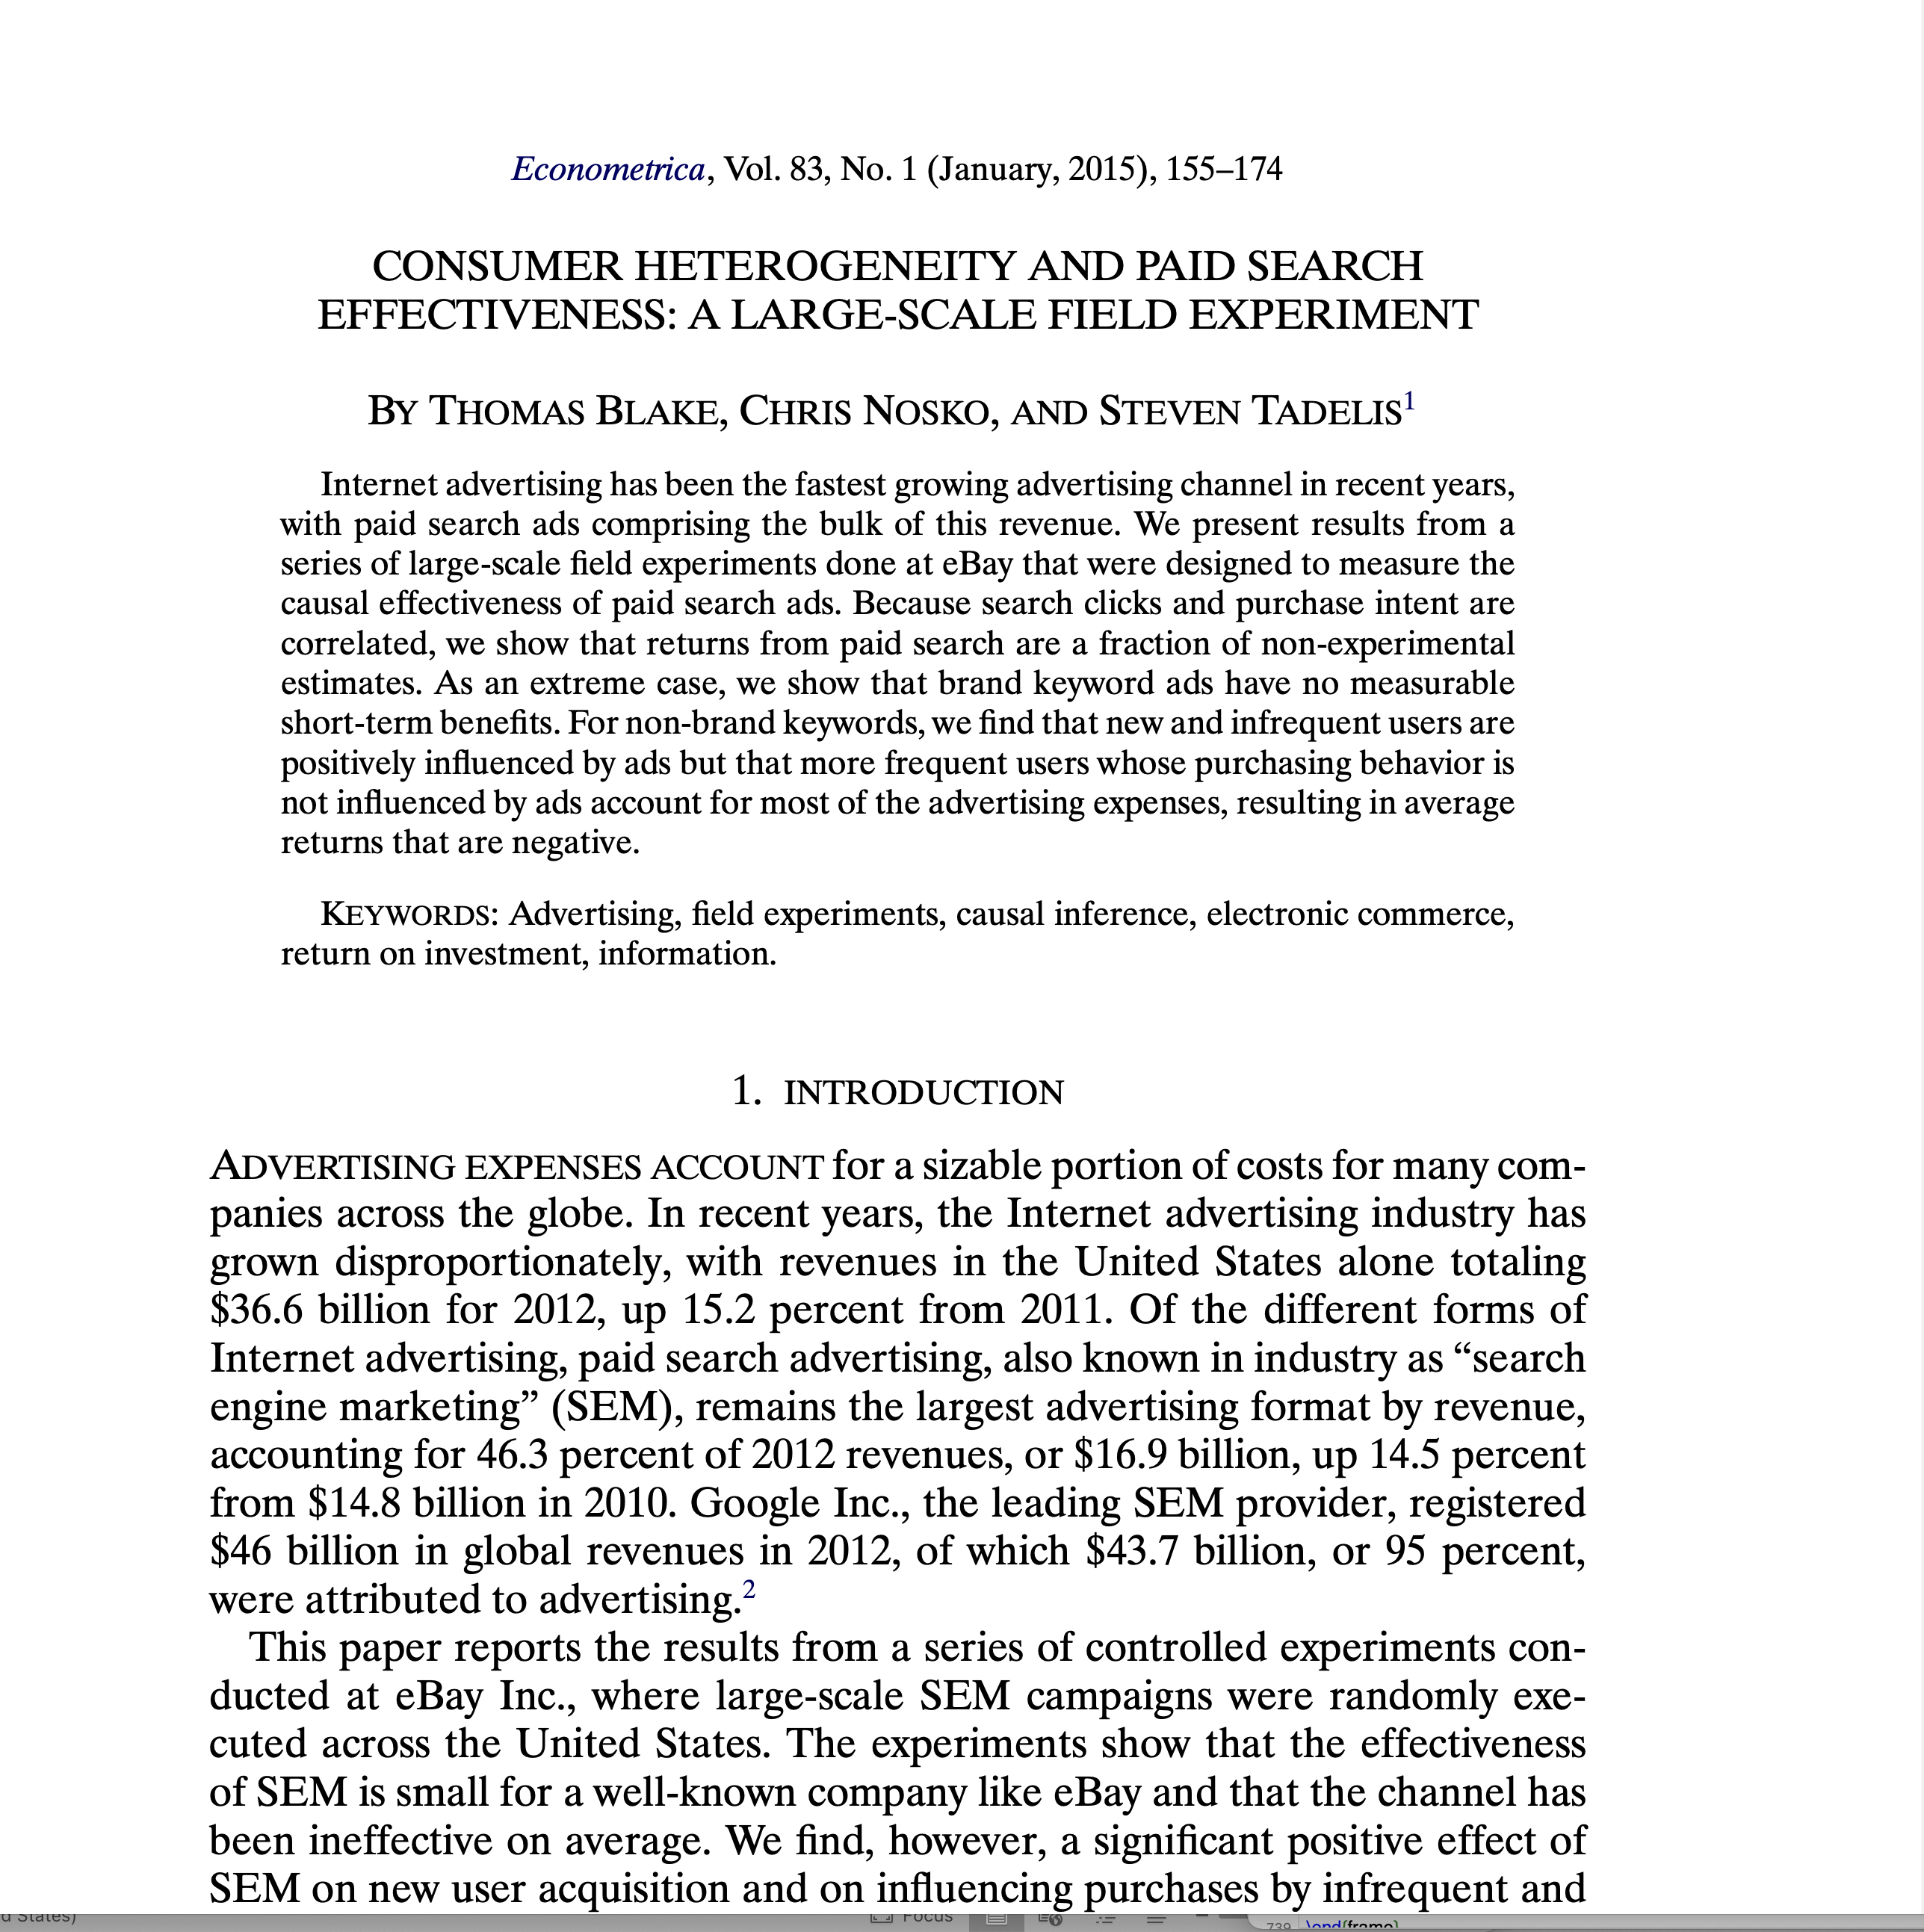
\includegraphics[scale=0.25]{./lecture_includes/econometrica_steve.png}
    \end{center}
  \end{figure}

\end{frame}

\begin{frame}{Internet advertising facts}

  \begin{itemize}
    \item In 2012, revenues from Internet advertising was \$36.6 billion and has only grown since
    \item Paid search (``search engine marketing'') is the largest format by revenue (46.3\% of 2012 revenues, or \$16.9 billion)
    \item Google is leading provider (registered \$46 billion in global revenues in 2012 of which 95\% was attributed to advertising)
  \end{itemize}

\end{frame}

\begin{frame}{Selection bias}

  \begin{itemize}
    \item Treatment was targeted ads at particular people conducting particular types of keyword search
    \item Consumers who choose to click on ads are loyal and already informed about products with high likelihood to buy already
    \item Problem is ads are targeting people at the end of their search, so the question is whether they would've found it already (i.e., $E[Y^0|D=1] \neq E[Y^0|D=0]$)
  \end{itemize}


\end{frame}



\begin{frame}{Selection bias}

  \begin{itemize}
    \item Estimated return on investment using OLS  found ROI of over 1600\%
    \item Compared this to experimental methods and found ROI of -63\% with a 95\% CI of $[-124\%, -3\%]$, rejecting the hypothesis that the channel yielded short-run positive returns
    \item Think back to perfect doctor -- Even without the treatment ($Y^0$), the treated group observationally would've still found a way
  \end{itemize}

\end{frame}

\begin{frame}{Natural experiment}

  \begin{itemize}
    \item Study began with a naturally occurring and somewhat fortuitous  event at eBay
    \item eBay halted SEM queries for brand words (i.e., queries that included the term eBay) on Yahoo! and Microsoft but continued to pay for these terms on Google
    \item Blake, Nosky and Tadelis (2015) showed almost all of the foregone click traffic and attributed sales were captured by natural search
    \item Substitution between paid and unpaid traffic was nearly one to one complete
  \end{itemize}

\end{frame}


\begin{frame}

  \begin{figure}
    \begin{center}
      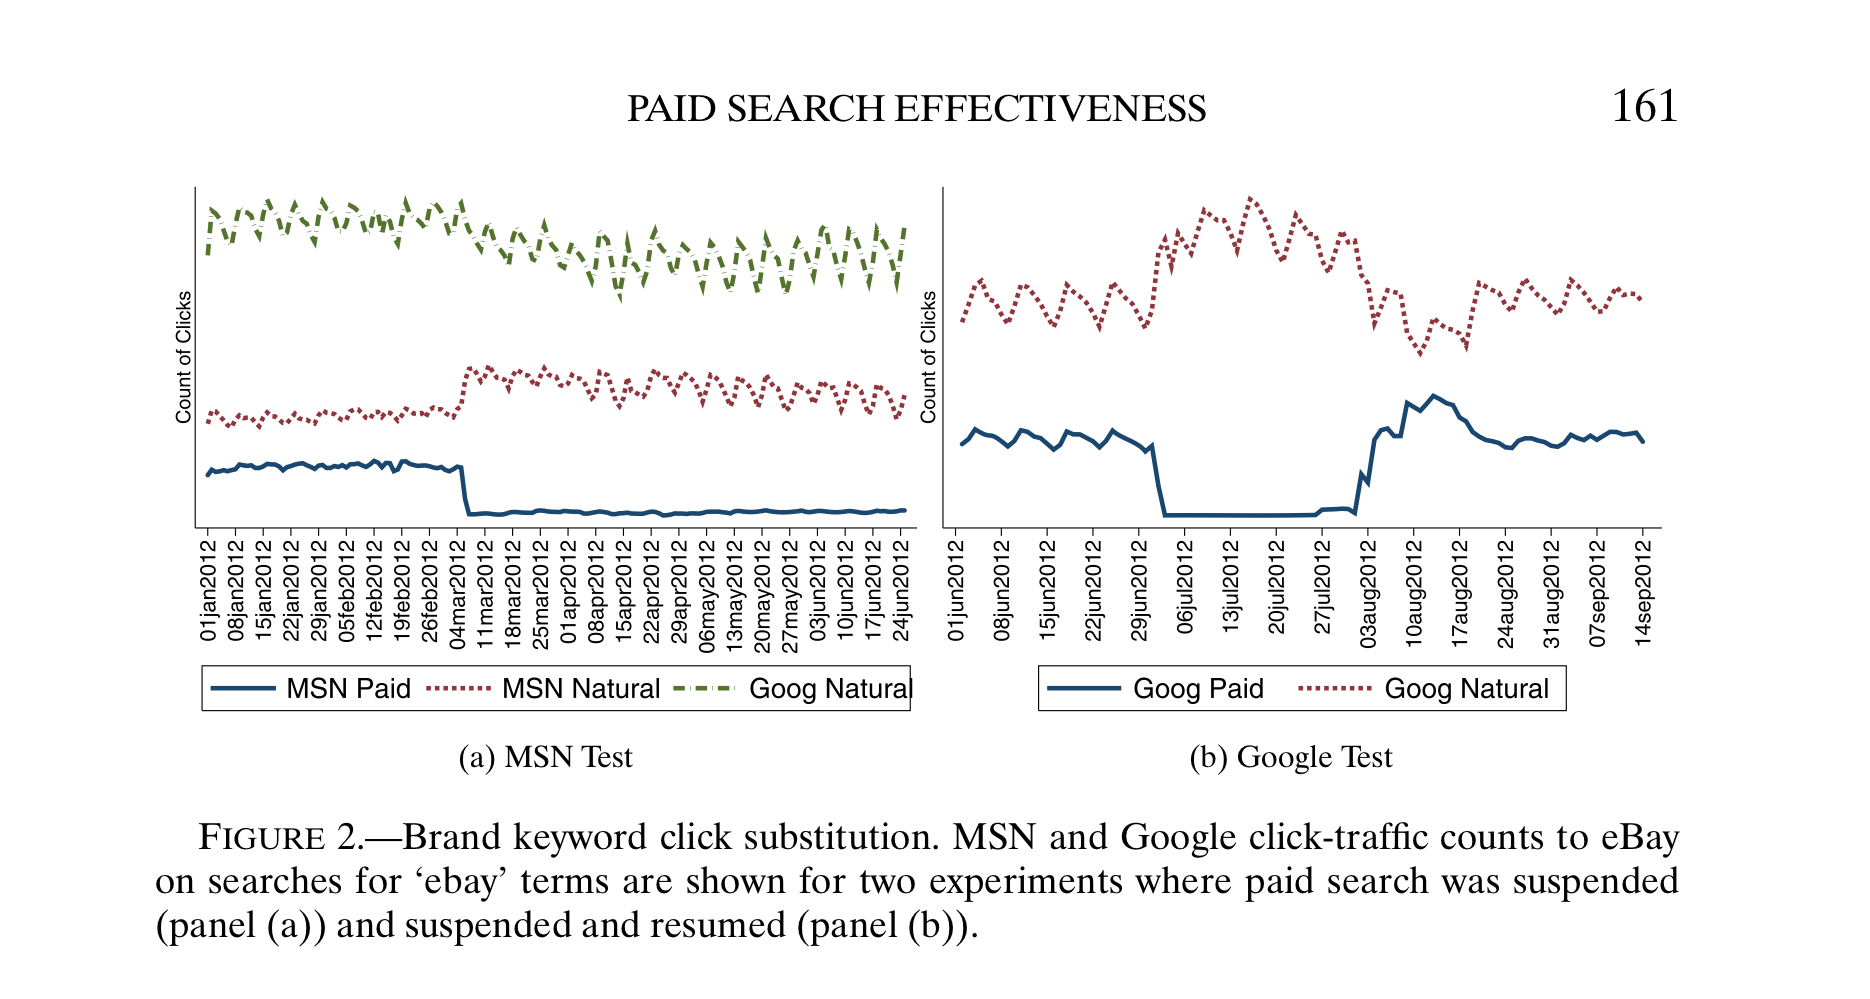
\includegraphics[scale=0.2]{./lecture_includes/tadelis_fig1.png}
    \end{center}
  \end{figure}

\end{frame}

\begin{frame}{Interpretation of natural experiment}

  \begin{quote}
    ``The evidence strongly supports the intuitive notion that for brand keywords, natural search is close to a perfect substitute for paid search, making brand keyword SEM ineffective for short-term sales.  After all, the users who type the brand keyword in the search query intend to reach the company's website, and most likely will execute on their intent regardless of the appearance of a paid search ad.''
  \end{quote}

\end{frame}

\begin{frame}{Selection bias}

  Observational data masked causal effect (recall the decomposition of the any non-designed estimation strategy)

  \bigskip

  \begin{quote}
    ``Advertising may appear to attract these consumers, when in reality they would have found other channels to visit the company's website.  We overcome this endogeneity challenge with our controlled experiments.''
  \end{quote}

\end{frame}




\begin{frame}{RCT}

  Natural experiment was valuable, but eBay could run a large scale RCT.

  \bigskip


  Use this finding of a nearly one-to-one substitution once paid search was dropped to convince eBay to field a large scale RCT discontinuing non-band key words

  \bigskip


\end{frame}

\begin{frame}{Design of the experiment}

  \begin{itemize}
    \item Randomly assigned 30 percent of eBay's US traffic to stop all bidding for all non-brand keywords for 60 days
    \item Some random group of users, in other words, were exposed to ads; a control group did not see the ads
    \item Used Google's geographic bid feature that can accurately identify geographic market of the user conducting the search
    \item Ads were suspended in 30 percent of markets to reduce the scope of the test and minimize the potential cost and impact to the business
  \end{itemize}

\end{frame}

\begin{frame}

  \begin{figure}
    \begin{center}
      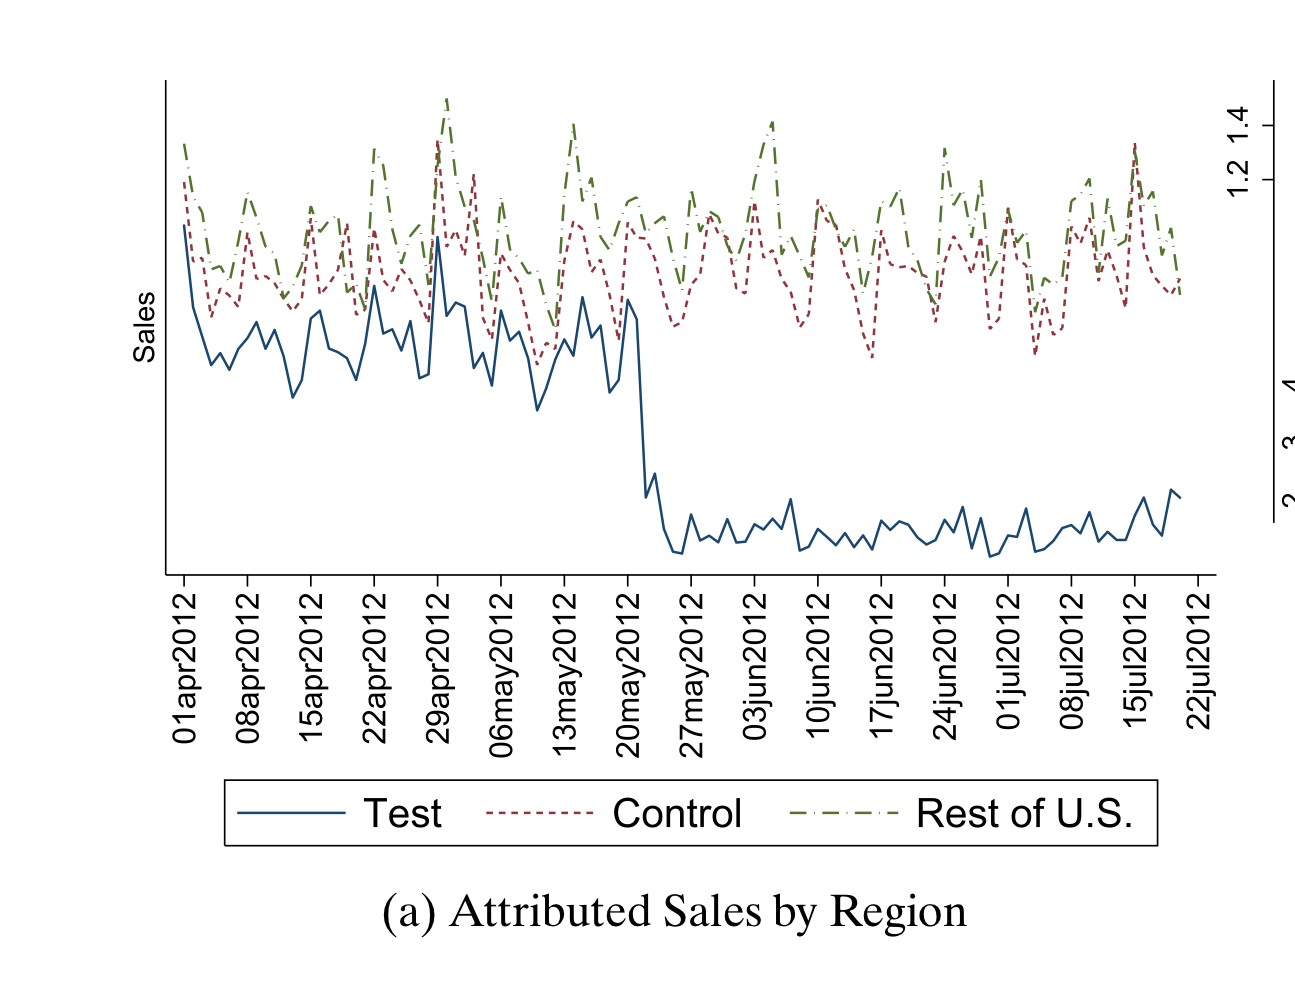
\includegraphics[scale=0.2]{./lecture_includes/tadelis_fig3.png}
      \caption{Attributed sales due to clicking on a Google link (treatment group)}
    \end{center}
  \end{figure}

\end{frame}


\begin{frame}

  \begin{figure}
    \begin{center}
      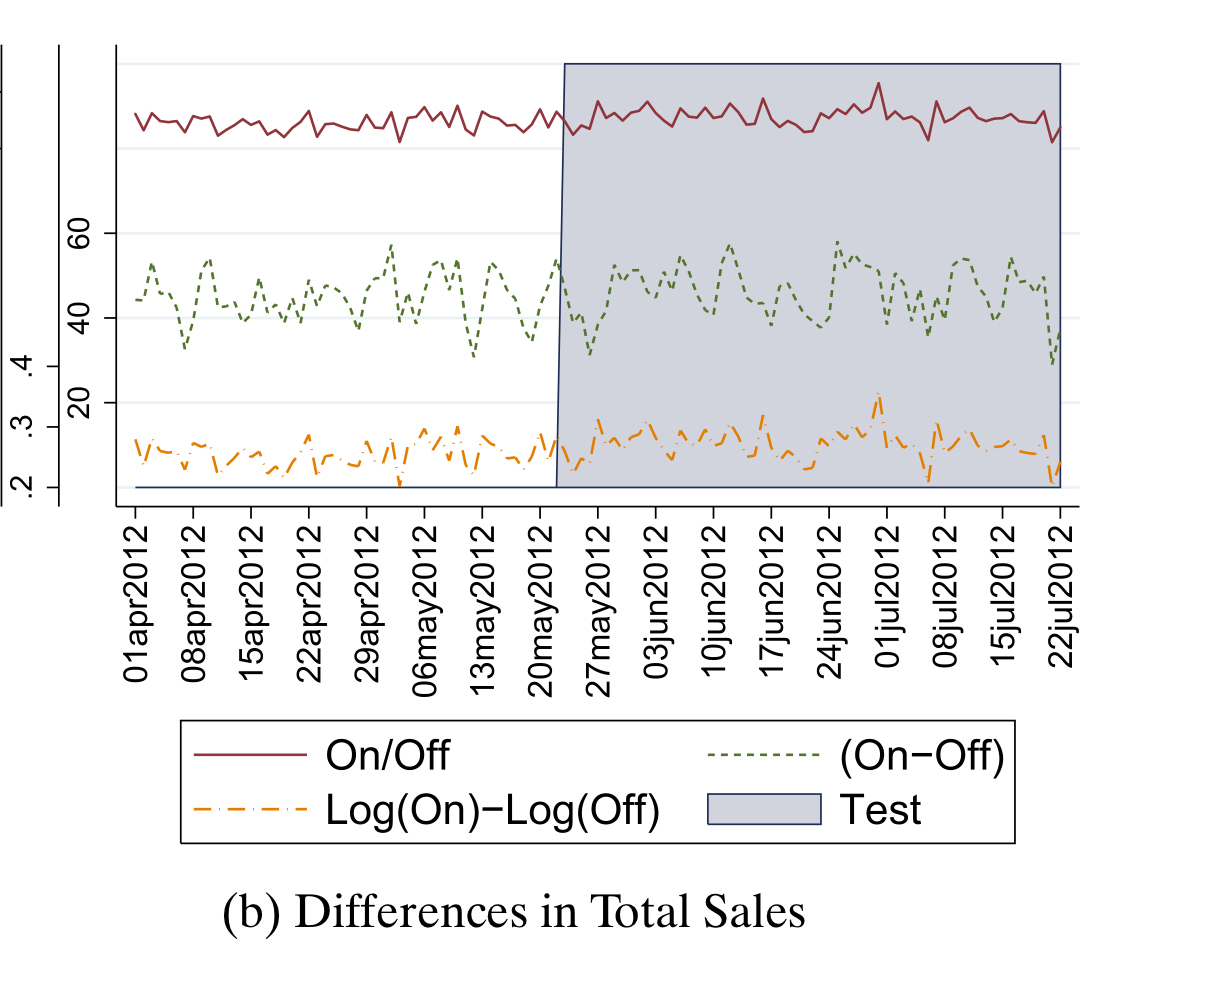
\includegraphics[scale=0.2]{./lecture_includes/tadelis_fig2.png}
      \caption{Differences in total sales by market (treatment to control)}
    \end{center}
  \end{figure}

\end{frame}

\begin{frame}

  \begin{figure}
    \begin{center}
      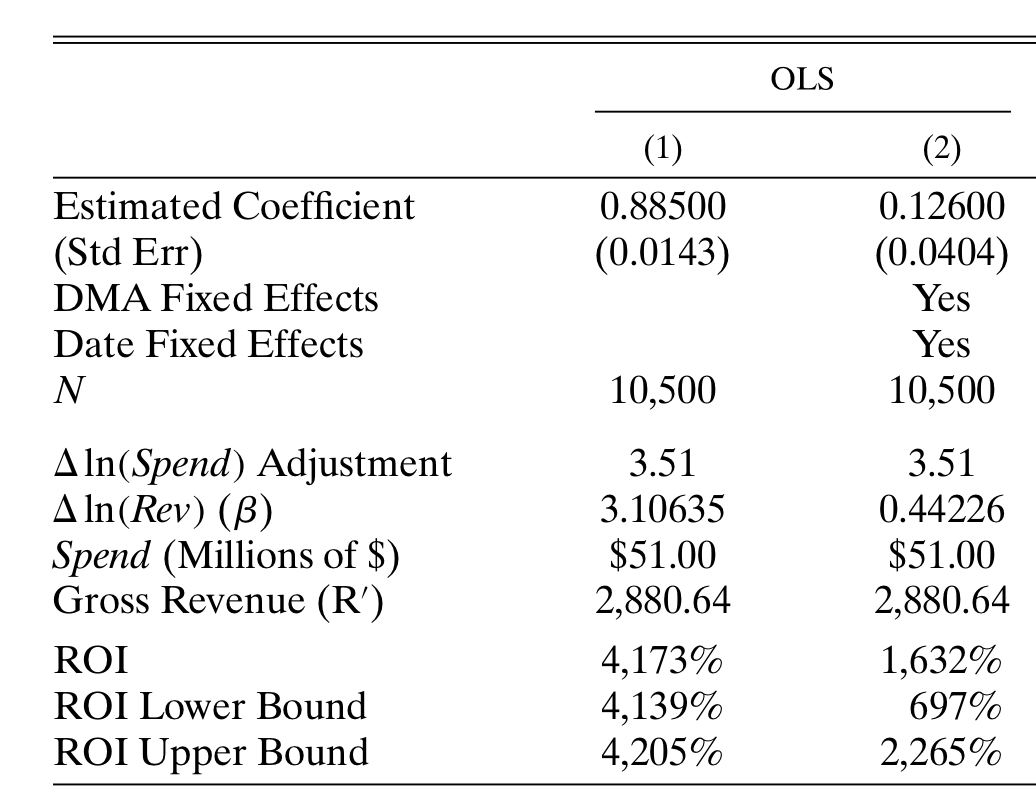
\includegraphics[scale=0.2]{./lecture_includes/tadelis_ols1.png}
      \caption{Spending effect on revenue using OLS but not the randomization. Effects are gigantic. }
    \end{center}
  \end{figure}

\end{frame}

\begin{frame}

  \begin{figure}
    \begin{center}
      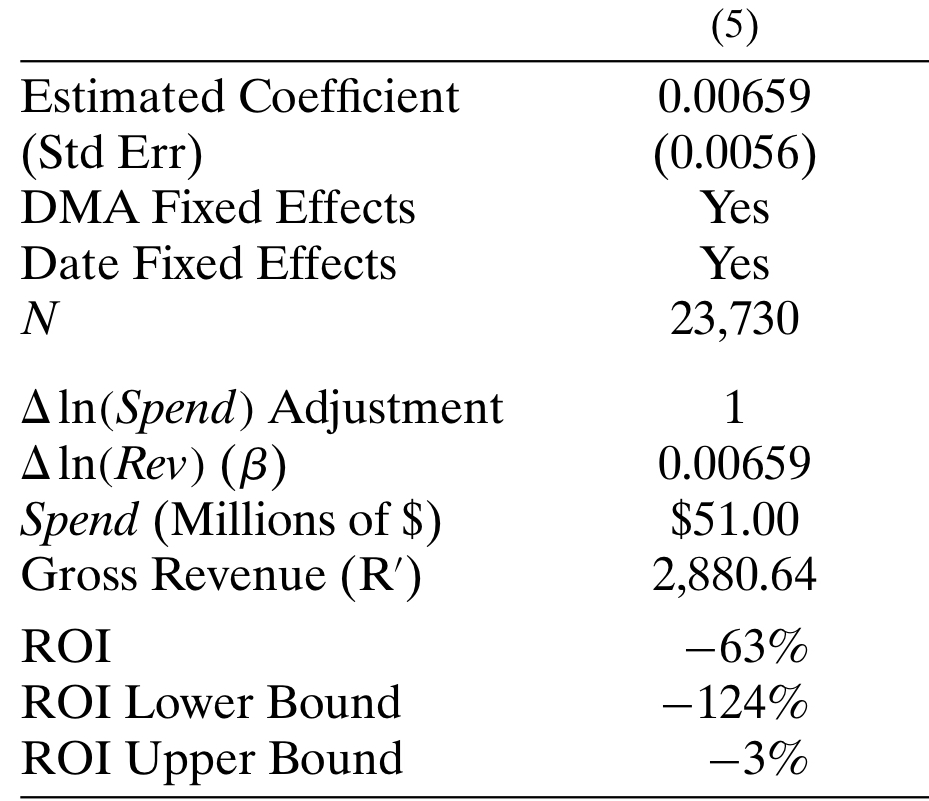
\includegraphics[scale=0.2]{./lecture_includes/tadelis_ols2.png}
      \caption{Spending effect on revenue using the randomization. Effects are negative. }
    \end{center}
  \end{figure}

\end{frame}

\begin{frame}{Heterogenous treatment effects}

  \begin{itemize}
    \item Recall how the potential outcomes model explicitly models individual treatment effects could be unique and that the perfect doctor showed selection on gains masked treatment effects, perhaps even reversing sign
    \item Search advertising in this RCT only worked if the consumer had no idea that the company had the desired product
    \item Large firms like eBay with powerful brands will see little benefit from paid search advertising because most consumers already know that they exist, as well as what they have to offer
  \end{itemize}

\end{frame}


\begin{frame}

  \begin{figure}
    \begin{center}
      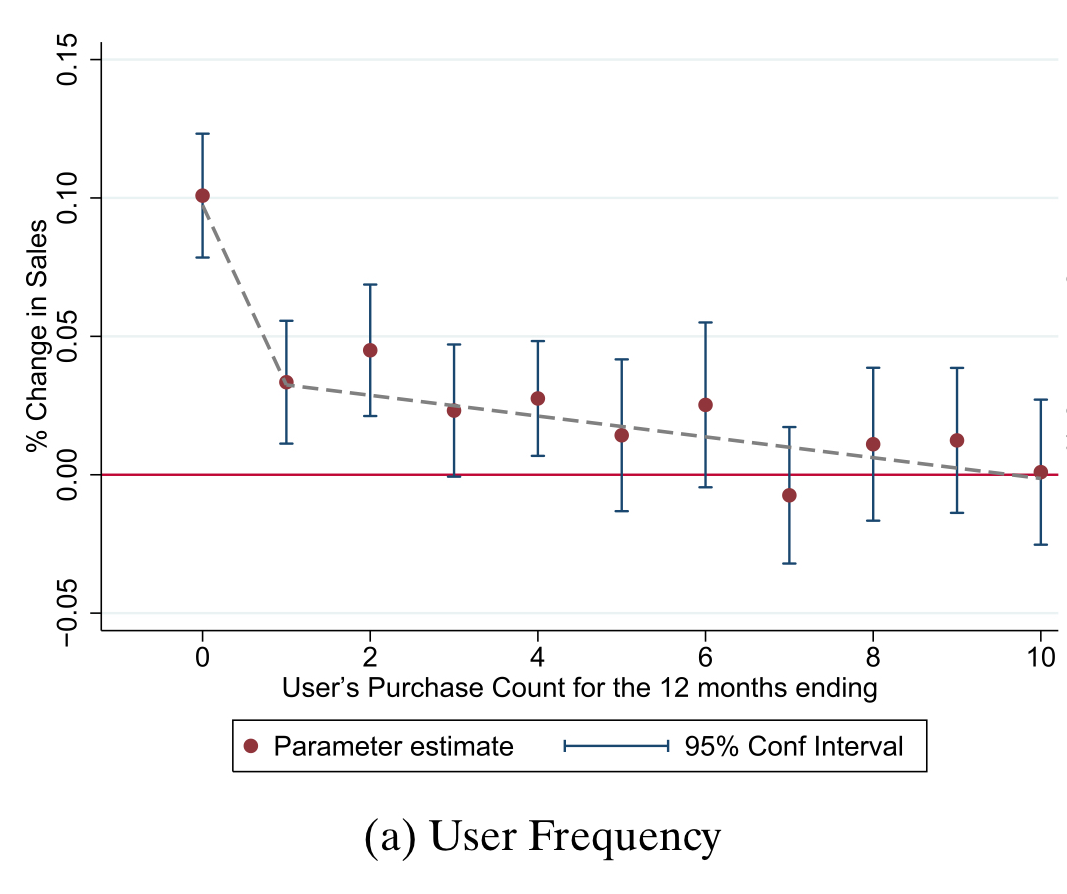
\includegraphics[scale=0.2]{./lecture_includes/tadelis_newuser_fig1.png}
      \caption{Effects on new users are positive and large, but not others. }
    \end{center}
  \end{figure}

\end{frame}

\begin{frame}

  \begin{figure}
    \begin{center}
      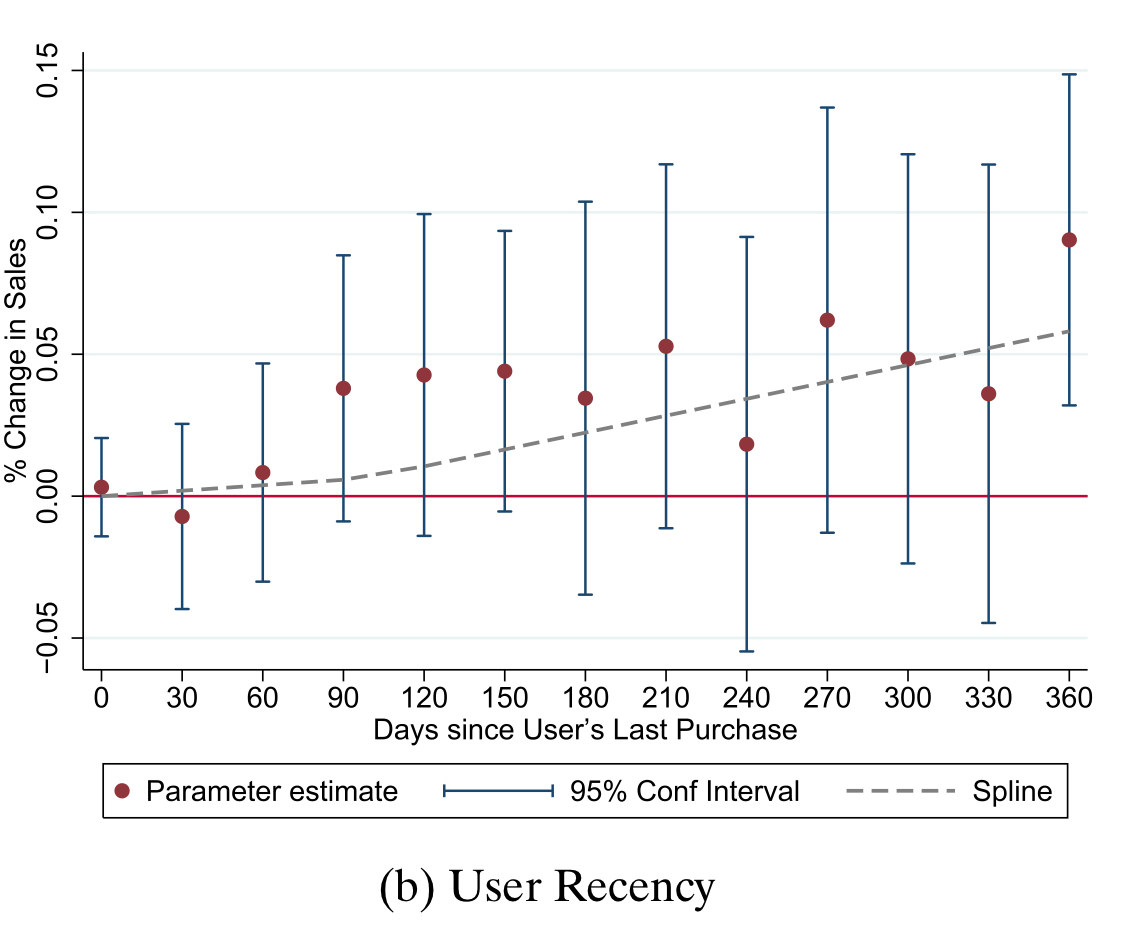
\includegraphics[scale=0.2]{./lecture_includes/tadelis_newuser_fig2.png}
      \caption{Effects are largest for ``least active'' customers. }
    \end{center}
  \end{figure}

\end{frame}


\begin{frame}{Why are causal effects small?}

  \begin{itemize}
    \item They suggest that the brand query tests found small causal returns because users simply substituted from the paid search clicks to the natural search clicks
    \item If that's the case, then it's explicitly a selection bias story $$E[Y^0|D=1] \neq E[Y^0|D=0]$$ where $D$ is being shown the branded advertisement based on search (i.e., they were already going there)
    \item They weren't using branded search for information; they were using to \emph{navigate}
  \end{itemize}

\end{frame}


\begin{frame}{Self selection based on gains}

  \begin{itemize}
    \item Potential outcomes is the foundation of the physical experiment because the physical experiment assigns units to treatments \emph{independent} of potential outcomes, $Y^0,Y^1$
    \item This is important because outside of the physical experiment, we expect people select those important treatments based on whether, subjectively, they think $Y^1>Y^0$ or $Y^1\leq Y^0$.
    \item Rational actors almost by definition are thought to ``self-select into treatment'' making non-designed comparisons potentially misleading -- sometimes by a little, sometimes by a lot
  \end{itemize}

\end{frame}

\begin{frame}{Natural experiments}

  \begin{itemize}
    \item Recall how Blake, et al. (2015) used that natural even in which eBay stopped paid search on two search engines but not Google?
    \item While the phrase ``natural experiment'' can be a misnomer, as these are not real experiments, it is nonetheless a helpful hook to hang your hat on as we go forward
    \item Natural experiments are important if the RCT we want to run may not be one we can run for any number of reasons
    \item Our course runs down alternative strategies, but each of them must replace independence with something else
    \item Separate in your minds identification from estimation -- it'll help as we progress
  \end{itemize}

\end{frame}

\subsection{Example of physical experimentation: HIV status}

\begin{frame}{Demand for Learning HIV Status}


  \begin{itemize}
    \item Rebecca Thornton implemented an RCT in rural Malawi for her job market paper at Harvard in mid-2000s
    \item At the time, it was an article of faith that you could fight the HIV epidemic in Africa by encouraging people to get tested; but Thornton wanted to see if this was true
    \item She randomly assigned cash incentives to people to incentivize learning their HIV status
    \item Also examined whether learning changed sexual behavior.
  \end{itemize}

\end{frame}

\begin{frame}{Experimental design}

  \begin{itemize}
    \item Respondents were offered a free door-to-door HIV test
    \item Treatment is randomized vouchers worth between zero and three dollars
    \item These vouchers were redeemable once they visited a nearby voluntary counseling and testing center (VCT)
    \item Estimates her models using OLS with controls
  \end{itemize}

\end{frame}


\begin{frame}{Why Include Control Variables?}

  To evaluate experimental data, one may want to add additional controls in the multivariate regression model.  So, instead of estimating the SDO, we might estimate:
  \begin{eqnarray*}
    Y_i = \alpha + \delta D_i + \gamma X_i + \eta_i
  \end{eqnarray*}
\end{frame}


\begin{frame}{Why Control Variables?}
  \begin{itemize}
    \item There are 2 main reasons for including additional controls in the regression models:
          \begin{enumerate}
            \item Conditional random assignment.  Sometimes randomization is done \emph{conditional} on some observable (e.g., gender, school, districts)
            \item Exogenous controls increase precision.  Although control variables $X_i$ are uncorrelated with $D_i$, they may have substantial explanatory power for $Y_i$. Including controls thus reduces variance in the residuals which lowers the standard errors of the regression estimates.
          \end{enumerate}
    \item Ongoing work by econometricians is investigating this more carefully
  \end{itemize}
\end{frame}



\begin{frame}[plain]
  \begin{table}[htbp]\centering
    \scriptsize
    \caption{Impact of Monetary Incentives and Distance on Learning HIV Results}
    \label{tab:thornton_main}
    \centering
    \begin{threeparttable}
      \begin{tabular}{l*{5}{c}}
        \toprule
        \multicolumn{1}{l}{\textbf{}}&
        \multicolumn{1}{c}{\textbf{1}}&
        \multicolumn{1}{c}{\textbf{2}}&
        \multicolumn{1}{c}{\textbf{3}}&
        \multicolumn{1}{c}{\textbf{4}}&
        \multicolumn{1}{c}{\textbf{5}}\\
        \midrule
        Any incentive           & 0.431***  & 0.309*** & 0.219***    & 0.220***    & 0.219 ***
        \\
                                & (0.023)   & (0.026)  & (0.029)     & (0.029)     & (0.029)
        \\
        Amount of incentive     &           & 0.091*** & 0.274***    & 0.274***    & 0.273***
        \\
                                &           & (0.012)  & (0.036)     & (0.035)     & (0.036)
        \\
        Amount of incentive$^2$ &           &          & $-0.063$*** & $-0.063$*** & $-0.063$***
        \\
                                &           &          & (0.011)     & (0.011)     & (0.011)
        \\
        HIV                     & $-0.055$* & $-0.052$ & $-0.05$     & $-0.058$*   & $-0.055$*   \\
                                & (0.031)   & (0.032)  & (0.032)     & (0.031)     & (0.031)
        \\
        Distance (km)           &           &          &             & $-0.076$*** &
        \\
                                &           &          &             & (0.027)     &             \\
        Distance$^2$            &           &          &             & 0.010**     &
        \\
                                &           &          &             & (0.005)     &
        \\\midrule
        Controls                & Yes       & Yes      & Yes         & Yes         & Yes
        \\
        Sample size             & 2,812     & 2,812    & 2,812       & 2,812       & 2,812
        \\
        Average attendance      & 0.69      & 0.69     & 0.69        & 0.69        & 0.69
        \\
        \bottomrule
      \end{tabular}
    \end{threeparttable}
  \end{table}

\end{frame}

\begin{frame}[plain]

  \begin{figure}[htb]\centering
    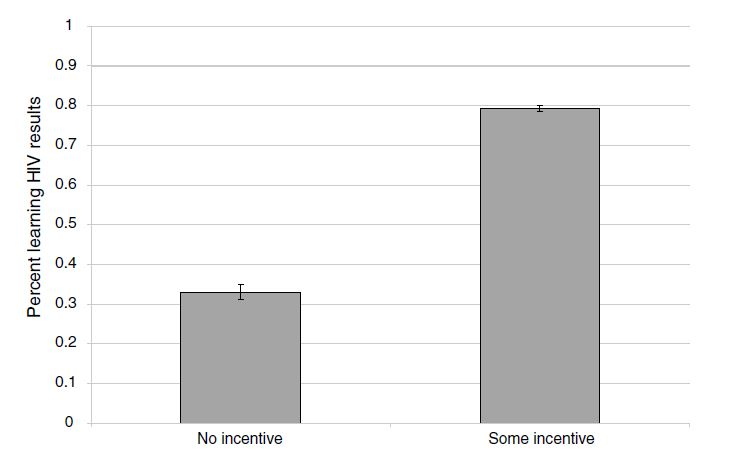
\includegraphics[scale=0.5]{./lecture_includes/FigA.jpg}
    \caption{Visual representation of cash transfers on learning HIV test results.}
    \label{fig:thorntonfig}
  \end{figure}

\end{frame}


\begin{frame}{Results}

  \begin{itemize}
    \item Even small incentives were effective
    \item Any incentive increases learning HIV status by 43\% compared to the control (mean 34\%)
    \item Next she looks at the effect that learning HIV status has on risky sexual behavior
  \end{itemize}

\end{frame}

\begin{frame}[plain]

  \begin{figure}[htb]\centering
    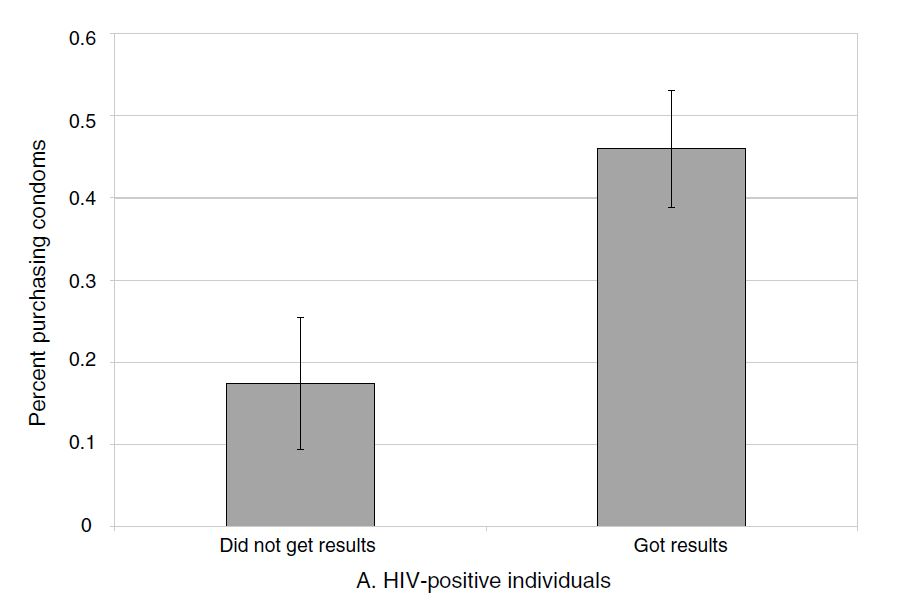
\includegraphics[scale=0.5]{./lecture_includes/FigC.jpg}
    \caption{Visual representation of cash transfers on condom purchases for HIV positive individuals.}
    \label{fig:thorntoncondomfig}
  \end{figure}

\end{frame}

\begin{frame}[plain]

  \begin{table}[htb]\centering
    \scriptsize
    \caption{Reactions to Learning HIV Results among Sexually Active at Baseline}
    \label{tab:thornton_condoms}
    \centering
    \begin{threeparttable}
      \begin{tabular}{l*{5}{c}}
        \toprule
        \multicolumn{1}{l}{\textbf{Dependent variables:}}&
        \multicolumn{2}{c}{\textbf{Bought}}&
        \multicolumn{2}{c}{\textbf{Number of}}\\
        \multicolumn{1}{l}{}&
        \multicolumn{2}{c}{\textbf{condoms}}&
        \multicolumn{2}{c}{\textbf{condoms bought}}\\
        \multicolumn{1}{l}{}&
        \multicolumn{1}{c}{\textbf{OLS}}&
        \multicolumn{1}{c}{\textbf{IV}}&
        \multicolumn{1}{c}{\textbf{OLS}}&
        \multicolumn{1}{c}{\textbf{IV}}\\
        \midrule
        Got results              & $-0.022$   & $-0.069$ & $-0.193$ & $-0.303$
        \\
                                 & (0.025)    & (0.062)  & (0.148)  & (0.285)
        \\
        Got results $\times$ HIV & 0.418***   & 0.248    & 1.778*** & 1.689**
        \\
                                 & (0.143)    & (0.169)  & (0.564)  & (0.784)  \\
        HIV                      & $-0.175$** & $-0.073$ & $-0.873$ & $-0.831$
        \\
                                 & (0.085)    & (0.123)  & (0.275)  & (0.375)  \\\midrule
        Controls                 & Yes        & Yes      & Yes      & Yes
        \\
        Sample size              & 1,008      & 1,008    & 1,008    & 1,008    \\
        Mean                     & 0.26       & 0.26     & 0.95     & 0.95     \\
        \bottomrule
      \end{tabular}
    \end{threeparttable}
  \end{table}

\end{frame}

\begin{frame}{Results}

  \begin{itemize}
    \item For those who were HIV$+$ and got their test results, 42\% more likely to buy condoms (but shrinks and becomes insignificant at conventional levels with IV).
    \item Number of condoms bought -- very small. HIV$+$ respondents who learned their status bought 2 more condoms
  \end{itemize}

\end{frame}

\begin{frame}{Discussion}

  \begin{itemize}
    \item What's in your field a causal question you find interesting that you wish you could answer?
    \item Describe the way you would conduct the RCT by explaining the following:
          \begin{itemize}
            \item What's the treatment?  Express it as a binary variable.
            \item How will you assign this so that SUTVA holds and independence is achieved?
            \item What is the outcome you are interested in?
          \end{itemize}
    \item Describe the steps you would take to do this if you had all the money in the world
  \end{itemize}

\end{frame}


\section{Directed Acyclic Graphs}

\subsection{Graph notation}

\begin{frame}{Judea Pearl, 2011 Turing Award winner, drinking his first IPA}

  \begin{figure}
    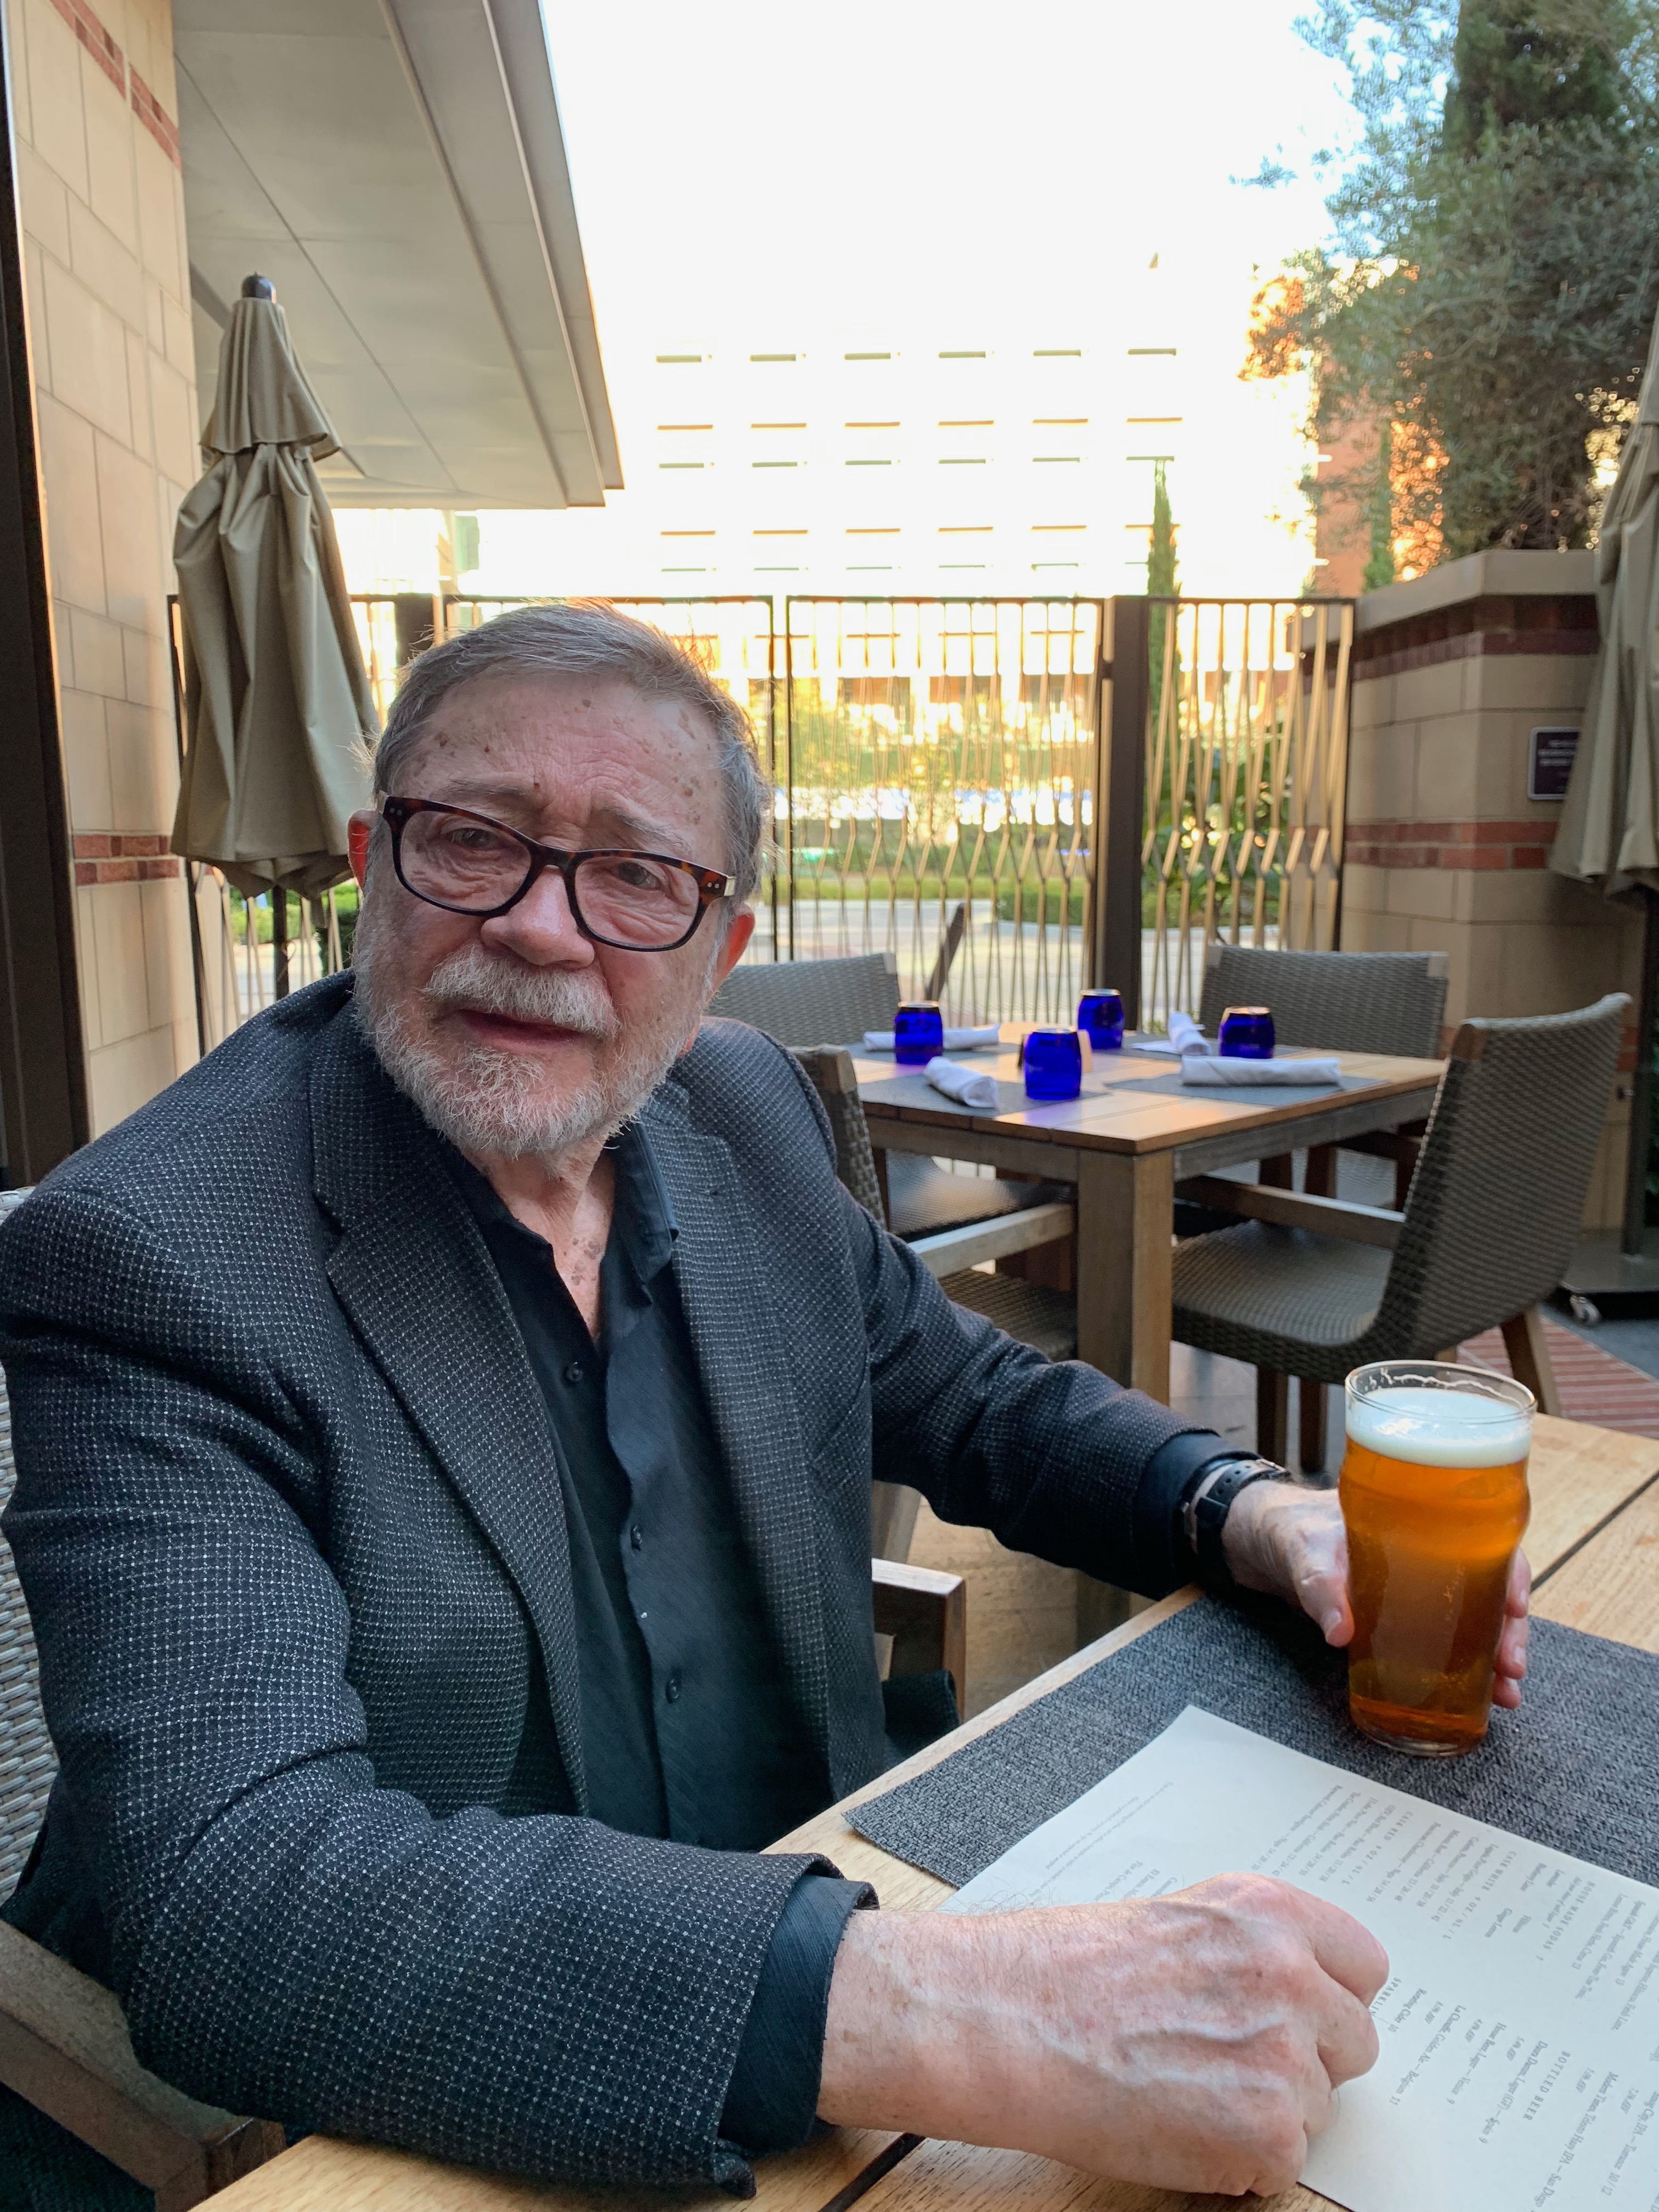
\includegraphics[scale=0.05]{./lecture_includes/pearl_ipa.jpg}
  \end{figure}

\end{frame}


\begin{frame}{Judea Pearl and DAGs}


  \begin{itemize}
    \item Judea Pearl and colleagues in Artificial Intelligence at UCLA developed DAG modeling to create a formalized causal inference methodology
    \item They causality concepts extremely clear, they provide a map to the estimation strategy, and maybe best of all, they communicate to others what must be true about the data generating process to recover the causal effect
  \end{itemize}

\end{frame}


\begin{frame}{Further reading}

  \begin{enumerate}

    \item Pearl (2018) \underline{The Book of Why: The} \underline{New Science of Cause and Effect}, Basic Books (\emph{popular})
    \item Morgan and Winship (2014) \underline{Counterfactuals and Causal Inference: Methods and Principles} \underline{for Social Research}, Cambridge University Press, 2nd edition (\emph{excellent})
    \item Pearl, Glymour and Jewell (2016) \underline{Causal Inference In Statistics: A Primer}, Wiley Books (\emph{accessible})
    \item Pearl (2009) \underline{Causality: Models, Reasoning and Inference}, Cambridge, 2nd edition (\emph{difficult})
    \item Cunningham (2021) \underline{Causal Inference: The Mixtape}, Yale, 1st edition (\emph{best choice, no question})
  \end{enumerate}

\end{frame}

\begin{frame}{Design vs. Model}

  \begin{itemize}
    \item DAGs tend to be focused more on the theory of treatment assignment in the world
    \item As such it's compatible with design-based approaches
    \item But assumptions in design based approaches tend to emphasize selection into treatment which is not exactly what is meant here
  \end{itemize}

\end{frame}

\begin{frame}{Causal model}

  \begin{itemize}
    \item The causal model is sometimes called the structural model, but for us, I prefer the former as it's less alienating
    \item Think of this as more connected to the model-based approach discussed earlier
    \item It's the system of equations describing the relevant aspects of the world
    \item It necessarily is filled with causal effects associated with some particular comparative statics
  \end{itemize}

\end{frame}

\begin{frame}[plain]

  \begin{center}
    \begin{tikzpicture}[node distance=1.5cm]
      % nodes %
      \node[text centered] (d) {$D$};
      \node[right of = d, text centered] (y) {$Y$};
      \node[above left of = d, text centered] (i) {$I$};
      \node[left of = i, text centered] (pe) {$PE$};
      \node[below of = pe, text centered] (b) {$B$};
      % edges %
      \draw[->, line width= 1] (d) -- (y);
      \draw[->, line width= 1,] (i) -- (d);
      \draw[->, line width= 1,] (pe) -- (i);
      \draw[->, line width= 1,] (pe) -- (d);
      \draw[->, line width= 1, dashed] (b) -- (pe);
      \draw[->, line width= 1, dashed] (b) -- (d);
      \draw[->, line width= .5] (i) to [out=45,in=135, looseness=0.5] (y);
    \end{tikzpicture}
  \end{center}

  \bigskip
  \begin{itemize}
    \item $B$ is a \textbf{parent} of $PE$ and $D$
    \item $PE$ and $D$ are \textbf{descendants} of $B$
    \item There is a \textbf{direct (causal) path} from $D$ to $Y$
    \item There is a \textbf{mediated (causal) path} from $B$ to $Y$ through $D$
    \item There are four \textbf{paths} from $PE$ to $Y$ but none are direct, and one is unlike the others
  \end{itemize}
\end{frame}


\begin{frame}{Colliders}

  \begin{center}
    \begin{tikzpicture}[node distance=1.5cm]
      % nodes %
      \node[text centered] (d) {$D$};
      \node[right of = d, text centered] (y) {$Y$};
      \node[above left of = d, text centered] (i) {$I$};
      \node[left of = i, text centered] (pe) {$PE$};
      \node[below of = pe, text centered] (b) {$B$};
      % edges %
      \draw[->, line width= 1] (d) -- (y);
      \draw[->, line width= 1,] (i) -- (d);
      \draw[->, line width= 1,] (pe) -- (i);
      \draw[->, line width= 1,] (pe) -- (d);
      \draw[->, line width= 1, dashed] (b) -- (pe);
      \draw[->, line width= 1, dashed] (b) -- (d);
      \draw[->, line width= .5] (i) to [out=45,in=135, looseness=0.5] (y);
    \end{tikzpicture}
  \end{center}

  \bigskip

  Notice anything different with this DAG?  Look closely.
  \begin{itemize}

    \item $D$ is a \textbf{collider} along the path $B\rightarrow D\leftarrow I$ (i.e., ``colliding'' at $D$)
    \item $D$ is a \textbf{noncollider} along the path $B\rightarrow D\rightarrow Y$

  \end{itemize}

\end{frame}


\begin{frame}{Summarizing Value of DAGs}

  \begin{enumerate}
    \item Facilitates the task of designing identification strategy for estimating average causal effects
    \item Facilitates the task of testing compatibility of the model with your data
    \item Visualizes the identifying assumptions which opens up the model to critical scrutiny
  \end{enumerate}

\end{frame}

\begin{frame}{Creating DAGs}

  \begin{itemize}
    \item The DAG is a \emph{relevant} causal relationships describing the relationship between $D$ and $Y$
    \item It will include:
          \begin{itemize}
            \item All direct causal effects among the \emph{relevant} variables in the graph
            \item All common causes of any pair of \emph{relevant} variables in the graph
          \end{itemize}
    \item No need to model a dinosaur stepping on a bug causing in a million years some evolved created that impacted your decision to go to college
    \item We get ideas for DAGs from theory, models, observation, experience, prior studies, intuition
    \item Sometimes called the data generating process.
  \end{itemize}

\end{frame}



\subsection{Backdoor criterion}

\begin{frame}{Research designs: Selection on observables}

  \begin{itemize}

    \item DAGs help us understand the source of problems in our observational (non-experimental) data that make inferring causality hard
    \item But it also can help us see a way out (this whole class is a way out)
    \item First way out is the selection on observables research design, which is best described in causal graphs using the \textbf{backdoor criterion}
    \item Selection on observables is not technically difficult, but it does require a reasonable level of confidence in the DAG
  \end{itemize}

\end{frame}

\begin{frame}{Confounding}

  \begin{itemize}
    \item Omitted variable bias has a name in DAGs: ``confounding''
    \item Confounding occurs when when the treatment and the outcomes have a common cause or parent which creates spurious correlation between $D$ and $Y$

          \begin{center}
            \begin{tikzpicture}
              [node distance=1.5cm]
              % nodes %
              \node[text centered] (d) {$D$};
              \node[below right of = d, text centered] (x) {$X$};
              \node[above right of = x, text centered] (y) {$Y$};

              % edges %
              \draw[->, line width= 1] (d) -- (y);
              \draw[->, line width= 1] (x) -- (d);
              \draw[->, line width= 1] (x) -- (y);
            \end{tikzpicture}
          \end{center}

          The \emph{correlation} between $D$ and $Y$ no longer reflects the causal effect of $D$ on $Y$
  \end{itemize}
\end{frame}

\begin{frame}{Backdoor Paths}

  \begin{itemize}
    \item Confounding creates \textbf{backdoor paths} between treatment and outcome ($D\leftarrow X\rightarrow Y$) -- i.e., spurious correlations
    \item Not the same as mediation ($D \rightarrow X \rightarrow Y$)
    \item We can ``block'' backdoor paths by conditioning on the common cause $X$
    \item Once we condition on $X$, the correlation between $D$ and $Y$ estimates the causal effect of $D$ on $Y$
    \item Conditioning means calculating $E[Y|D=1,X]-E[Y|D=0,X]$ for each value of $X$ then combining (e.g., integrating)

  \end{itemize}

  \begin{center}
    \begin{tikzpicture}
      [node distance=1.5cm]
      % nodes %
      \node[text centered] (d) {$D$};
      \node[below right of = d, text centered, rectangle, draw, thin] (x) {$X$};
      \node[above right of = x, text centered] (y) {$Y$};

      % edges %
      \draw[->, line width= 1] (d) -- (y);
      \draw[->, line width= 1] (x) -- (d);
      \draw[->, line width= 1] (x) -- (y);
    \end{tikzpicture}
  \end{center}

\end{frame}


\begin{frame}{Blocked backdoor paths}

  A backdoor path is blocked if and only if:
  \begin{itemize}
    \item It contains a noncollider that has been conditioned on
    \item Or it contains a collider that has not been conditioned on
  \end{itemize}

\end{frame}


\begin{frame}{Examples of blocked paths}

  Examples:
  \begin{enumerate}
    \item Conditioning on a noncollider blocks a path:

          \begin{center}
            \begin{tikzpicture}
              [node distance=1.5cm]
              % nodes %
              \node[text centered, rectangle, draw, thin] (x) {$X$};
              \node[right of = x, text centered] (z) {$Z$};
              \node[right of = z, text centered] (y) {$Y$};

              % edges %
              \draw[->, line width= .5] (x) -- (z);
              \draw[->, line width= .5] (x) to [out=45,in=135, looseness=0.5] (y);
            \end{tikzpicture}
          \end{center}

    \item Conditioning on a collider opens a path (i.e., creates spurious correlations):

          \begin{center}
            \begin{tikzpicture}
              [node distance=1.5cm]
              % nodes %
              \node[text centered] (z) {$Z$};
              \node[right of = z, text centered, rectangle, draw, thin] (x) {$X$};
              \node[right of = x, text centered] (y) {$Y$};

              % edges %
              \draw[->, line width= .5] (z) -- (x);
              \draw[->, line width= .5] (y) -- (x);
            \end{tikzpicture}
          \end{center}

    \item \emph{Not} conditioning on a collider blocks a path:

          \begin{center}
            \begin{tikzpicture}
              [node distance=1.5cm]
              % nodes %
              \node[text centered] (z) {$Z$};
              \node[right of = z, text centered] (x) {$X$};
              \node[right of = x, text centered] (y) {$Y$};

              % edges %
              \draw[->, line width= .5] (z) -- (x);
              \draw[->, line width= .5] (y) -- (x);
            \end{tikzpicture}
          \end{center}

  \end{enumerate}
\end{frame}


\begin{frame}{Backdoor criterion}


  \begin{block}{Backdoor criterion}
    Conditioning on $X$ satisfies the backdoor criterion with respect to $(D,Y)$ directed path if:
    \begin{enumerate}
      \item All backdoor paths are blocked by $X$
      \item No element of $X$ is a collider
    \end{enumerate}

    In words: If $X$ satisfies the backdoor criterion with respect to $(D,Y)$, then controlling for or matching on $X$ identifies the causal effect of $D$ on $Y$
  \end{block}
\end{frame}

\begin{frame}{What control strategy meets the backdoor criterion?}
  \begin{itemize}
    \item List all backdoor paths from $D$ to $Y$. I'll wait.

          \begin{center}
            \begin{tikzpicture}
              [node distance=1.5cm]
              % nodes %
              \node[text centered,rectangle,thin] (x1) {$X_1$};
              \node[right of = x1, text centered] (d) {$D$};
              \node[below right of = d, text centered] (x2) {$X_2$};
              \node[above right of = x2, text centered] (y) {$Y$};

              % edges %
              \draw[->, line width= .5] (x1) -- (d);
              \draw[->, line width= .5] (d) -- (y);
              \draw[->, line width= .5] (x2) -- (d);
              \draw[->, line width= .5] (x2) -- (y);
              \draw[->, line width= .5] (x1) to [out=45,in=135, looseness=0.5] (y);
            \end{tikzpicture}
          \end{center}

    \item What are the necessary and sufficient set of controls which will satisfy the backdoor criterion?
  \end{itemize}

  \framebreak




\end{frame}


\begin{frame}{What if you have an unobservable?}


  \begin{itemize}
    \item List all the backdoor paths from $D$ to $Y$.

          \begin{center}
            \begin{tikzpicture}
              [node distance=1.5cm]
              % nodes %
              \node[text centered] (u) {$U$};
              \node[right of = u, text centered] (x2) {$X_2$};
              \node[above of = x2, text centered] (x1) {$X_1$};
              \node[right of = x2, text centered] (d) {$D$};
              \node[right of = d, text centered] (y) {$Y$};

              % edges %
              \draw[->, line width= .5, dashed] (u) -- (x2);
              \draw[->, line width= .5] (x2) -- (d);
              \draw[->, line width= .5] (x1) -- (d);
              \draw[->, line width= .5] (x1) -- (y);
              \draw[->, line width= .5] (d) -- (y);
              \draw[->, line width= .5, dashed] (u) to [out=-45,in=-135, looseness=0.5] (y);
            \end{tikzpicture}
          \end{center}

    \item What are the necessary and sufficient set of controls which will satisfy the backdoor criterion?
    \item What about the unobserved variable, $U$?
  \end{itemize}

  \framebreak


\end{frame}

\begin{frame}{Multiple strategies}


  \begin{center}
    \begin{tikzpicture}
      [node distance=1.5cm, text centered]
      % nodes %
      \node[] (x3) {$X_3$};
      \node[above left of = x3,rectangle,draw,thin] (x1) {$X_1$};
      \node[below left of = x3,rectangle,draw,thin] (x2) {$X_2$};
      \node[right of = x] (d) {$D$};
      \node[right of = d] (y) {$Y$};

      % edges %
      \draw[->, line width= .5] (x1) -- (x3);
      \draw[->, line width= .5] (x2) -- (x3);
      \draw[->, line width= .5] (x1) to [out=0,in=135, looseness=0.5] (y);
      \draw[->, line width= .5] (x2) to [out=0,in=-135, looseness=0.5] (y);
      \draw[->, line width= .5] (x3) -- (d);
      \draw[->, line width= .5] (d) -- (y);
    \end{tikzpicture}

    \begin{tikzpicture}
      [node distance=1.5cm, text centered]
      % nodes %
      \node[rectangle,draw,thin] (x3) {$X_3$};
      \node[above left of = x3] (x1) {$X_1$};
      \node[below left of = x3] (x2) {$X_2$};
      \node[right of = x] (d) {$D$};
      \node[right of = d] (y) {$Y$};

      % edges %
      \draw[->, line width= .5] (x1) -- (x3);
      \draw[->, line width= .5] (x2) -- (x3);
      \draw[->, line width= .5] (x1) to [out=0,in=135, looseness=0.5] (y);
      \draw[->, line width= .5] (x2) to [out=0,in=-135, looseness=0.5] (y);
      \draw[->, line width= .5] (x3) -- (d);
      \draw[->, line width= .5] (d) -- (y);
    \end{tikzpicture}
  \end{center}

  \begin{itemize}
    \item Conditioning on the common causes, $X_1$ and $X_2$, is sufficient
    \item \dots but so is conditioning on $X_3$
  \end{itemize}
\end{frame}

\begin{frame}{Testing the Validity of the DAG}

  \begin{itemize}
    \item The DAG makes testable predictions
    \item Conditional on $D$ and $I$, parental education ($PE$) should no longer be correlated with $Y$
    \item Can be hard to figure this out by hand, but software can help (e.g., Daggity.net is browser based, Causal Fusion is more advanced)
    \item Causal algorithms tend to be DAG based and are becoming popular in industry
  \end{itemize}

  \begin{center}
    \begin{tikzpicture}[node distance=1.5cm]
      % nodes %
      \node[text centered] (d) {$D$};
      \node[right of = d, text centered] (y) {$Y$};
      \node[above left of = d, text centered] (i) {$I$};
      \node[left of = i, text centered] (pe) {$PE$};
      \node[below of = pe, text centered] (b) {$B$};
      % edges %
      \draw[->, line width= 1] (d) -- (y);
      \draw[->, line width= 1,] (i) -- (d);
      \draw[->, line width= 1,] (pe) -- (i);
      \draw[->, line width= 1,] (pe) -- (d);
      \draw[->, line width= 1, dashed] (b) -- (pe);
      \draw[->, line width= 1, dashed] (b) -- (d);
      \draw[->, line width= .5] (i) to [out=45,in=135, looseness=0.5] (y);
    \end{tikzpicture}
  \end{center}

\end{frame}





\subsection{Collider bias}

\begin{frame}[allowframebreaks,plain]
  \begin{center}
    \textbf{Collider bias}
  \end{center}

  \begin{itemize}
    \item \textbf{Conditioning on a collider introduces spurious correlations; can even mask causal directions}
          \begin{itemize}
            \item There is only one backdoor path from $D$ to $Y$

                  \begin{center}
                    \begin{tikzpicture}
                      [node distance=1.5cm]
                      % nodes %
                      \node[text centered,draw,rectangle,thin] (x1) {$X_1$};
                      \node[right of = x1, text centered] (d) {$D$};
                      \node[below right of = d, text centered] (x2) {$X_2$};
                      \node[above right of = x2, text centered] (y) {$Y$};

                      % edges %
                      \draw[->, line width= .5] (x1) -- (d);
                      \draw[->, line width= .5] (d) -- (y);
                      \draw[->, line width= .5] (d) -- (x2);
                      \draw[->, line width= .5] (y) -- (x2);
                      \draw[->, line width= .5] (x1) to [out=45,in=135, looseness=0.5] (y);
                    \end{tikzpicture}
                  \end{center}

            \item Conditioning on $X_1$ blocks the backdoor path

            \item But what if we also condition on $X_2$?

                  \begin{center}
                    \begin{tikzpicture}
                      [node distance=1.5cm]
                      % nodes %
                      \node[text centered,draw,rectangle,thin] (x1) {$X_1$};
                      \node[right of = x1, text centered] (d) {$D$};
                      \node[below right of = d, draw, rectangle, text centered] (x2) {$X_2$};
                      \node[above right of = x2, text centered] (y) {$Y$};

                      % edges %
                      \draw[->, line width= .5] (x1) -- (d);
                      \draw[->, line width= .5] (d) -- (y);
                      \draw[->, line width= .5] (d) -- (x2);
                      \draw[->, line width= .5] (y) -- (x2);
                      \draw[->, line width= .5] (x1) to [out=45,in=135, looseness=0.5] (y);
                    \end{tikzpicture}
                  \end{center}

            \item Conditioning on $X_2$ opens up a new path, creating new spurious correlations between $D$ and $Y$
          \end{itemize}

          \framebreak


    \item \textbf{Even controlling for pretreatment covariates can create bias}
          \begin{itemize}
            \item Name the backdoor paths.  Is it open or closed?

                  \begin{center}
                    \begin{tikzpicture}
                      [node distance=1.5cm, text centered]
                      % nodes %
                      \node[] (x) {$X$};
                      \node[above left of = x] (u1) {$U_1$};
                      \node[below left of = x] (u2) {$U_2$};
                      \node[right of = x] (d) {$D$};
                      \node[right of = d] (y) {$Y$};

                      % edges %
                      \draw[->, line width= .5, dashed] (u1) -- (x);
                      \draw[->, line width= .5, dashed] (u2) -- (x);
                      \draw[->, line width= .5, dashed] (u1) to [out=0,in=135, looseness=0.5] (y);
                      \draw[->, line width= .5, dashed] (u2) to [out=0,in=-135, looseness=0.5] (d);
                      \draw[->, line width= .5] (d) -- (y);
                    \end{tikzpicture}
                  \end{center}

            \item But what if we condition on $X$?

                  \begin{center}
                    \begin{tikzpicture}
                      [node distance=1.5cm, text centered]
                      % nodes %
                      \node[text centered,draw,rectangle,thin] (x) {$X$};
                      \node[above left of = x] (u1) {$U_1$};
                      \node[below left of = x] (u2) {$U_2$};
                      \node[right of = x] (d) {$D$};
                      \node[right of = d] (y) {$Y$};

                      % edges %
                      \draw[->, line width= .5, dashed] (u1) -- (x);
                      \draw[->, line width= .5, dashed] (u2) -- (x);
                      \draw[->, line width= .5, dashed] (u1) to [out=0,in=135, looseness=0.5] (y);
                      \draw[->, line width= .5, dashed] (u2) to [out=0,in=-135, looseness=0.5] (d);
                      \draw[->, line width= .5] (d) -- (y);
                    \end{tikzpicture}
                  \end{center}


          \end{itemize}
  \end{itemize}
  \framebreak


\end{frame}


\begin{frame}{Sample selection example of collider bias}

  \alert{Important}: Since unconditioned colliders block back-door paths, what exactly does conditioning on a collider do? Let's illustrate with a fun example and some made-up data\\
  \begin{itemize}
    \item \underline{CNN.com} headline: Megan Fox voted worst -- but sexiest -- actress of 2009 \myurlshort{http://marquee.blogs.cnn.com/2009/12/30/megan-fox-voted-worst-but-sexiest-actress-of-2009/}{(link)}
    \item Are these two things actually negatively correlated in the world?
    \item Assume talent and beauty are independent, but each causes someone to become a movie star.  What's the correlation between talent and beauty for a sample of movie stars compared to the population as a whole (stars and non-stars)?
  \end{itemize}

\end{frame}


\begin{frame}[plain]

  \begin{itemize}
    \item What if the sample consists \emph{only} of movie stars?
    \item Look at python code
  \end{itemize}

  \begin{center}
    \begin{tikzpicture}
      [node distance=2cm, text centered]

      %nodes
      \node[text centered,draw,rectangle,thin] (x) {Movie Star};
      \node[below left of = x] (u1) {$Talent$};
      \node[below right of = x] (u2) {$Beauty$};

      % edges %
      \draw[->, line width= 2] (u1) -- (x);
      \draw[->, line width= 2] (u2) -- (x);
    \end{tikzpicture}
  \end{center}




\end{frame}

\begin{frame}[shrink=20,plain]

  \begin{figure}
    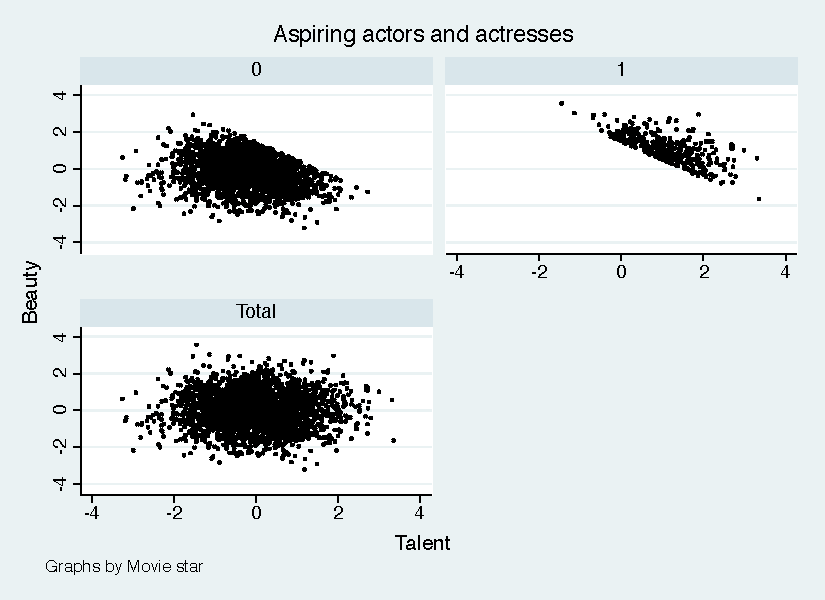
\includegraphics[height=9cm]{./lecture_includes/beauty_collider.pdf}
    \caption{Top left figure: Non-star sample scatter plot of beauty (vertical axis) and talent (horizontal axis). Top right right figure: Star sample scatter plot of beauty and talent.  Bottom left figure: Entire (stars and non-stars combined) sample scatter plot of beauty and talent.}
  \end{figure}
\end{frame}


\begin{frame}{Occupational sorting and discrimination example of collider bias}

  \begin{itemize}
    \item Let's look at another example: very common for think tanks and journalists to say that the gender gap in earnings disappears once you control for occupation.
    \item But what if occupation is a collider, which it could be in a model with occupational sorting
    \item Then controlling for occupation in a wage regression searching for discrimination can lead to all kinds of crazy results \emph{even in a simulation where we explicitly design there to be discrimination}
  \end{itemize}

\end{frame}

\begin{frame}{DAG}

  \begin{center}
    \begin{tikzpicture}
      [node distance=1.5cm]
      % nodes %
      \node[text centered] (f) {$F$};
      \node[above right of = f, text centered] (d) {$d$};
      \node[right of = f] (y) {$y$};
      \node[below  of = f, text centered] (o) {$o$};
      \node[right of = o, text centered] (a) {$A$};

      % edges %
      \draw[->, line width= 1] (f) -- (d);
      \draw[->, line width= 1] (d) -- (o);
      \draw[->, line width= 1, dashed] (a) -- (o);

      \draw[->, line width= 1] (d) -- (y);
      \draw[->, line width= 1] (o) -- (y);
      \draw[->, line width= 1, dashed] (a) -- (y);

    \end{tikzpicture}
  \end{center}

  $F$ is female, $d$ is discrimination, $o$ is occupation, $y$ is earnings and $A$ is ability. Dashed lines mean the variable cannot be observed. Note, by design, being a female has no effect on earnings or occupation, and has no relationship with ability. So earnings is coming through discrimination, occupation, and ability.

\end{frame}


\begin{frame}[plain]

  \begin{center}
    \begin{tikzpicture}
      [node distance=1.5cm]
      % nodes %
      \node[text centered] (f) {$F$};
      \node[above right of = f, text centered] (d) {$d$};
      \node[right of = f] (y) {$y$};
      \node[below  of = f, text centered] (o) {$o$};
      \node[right of = o, text centered] (a) {$A$};

      % edges %
      \draw[->, line width= 1] (f) -- (d);
      \draw[->, line width= 1] (d) -- (o);
      \draw[->, line width= 1, dashed] (a) -- (o);

      \draw[->, line width= 1] (d) -- (y);
      \draw[->, line width= 1] (o) -- (y);
      \draw[->, line width= 1, dashed] (a) -- (y);

    \end{tikzpicture}
  \end{center}


  Mediation and Backdoor paths

  \begin{enumerate}

    \item $d$ $\rightarrow o \rightarrow y$
    \item $d$ $\rightarrow o \leftarrow A \rightarrow y$
  \end{enumerate}

\end{frame}


\begin{frame}[plain, shrink=20]

  \begin{table}[htbp]\centering
    \scriptsize
    \caption{Regressions illustrating collider bias with simulated gender disparity}
    \begin{center}
      \begin{tabular}{l*{3}{c}}
        \toprule
        \multicolumn{1}{l}{Covariates: }&
        \multicolumn{1}{c}{\textbf{Unbiased combined effect}}&
        \multicolumn{1}{c}{\textbf{Biased }}&
        \multicolumn{1}{c}{\textbf{Unbiased wage effect only}}\\
        \midrule
        Female                     & -3.074*** & 0.601*** & -0.994*** \\
                                   & (0.000)   & (0.000)  & (0.000)   \\
        Occupation                 &           & 1.793*** & 0.991***  \\
                                   &           & (0.000)  & (0.000)   \\
        Ability                    &           &          & 2.017***  \\
                                   &           &          & (0.000)   \\
        \\
        \midrule
        N                          & 10,000    & 10,000   & 10,000    \\
        Mean of dependent variable & 0.45      & 0.45     & 0.45      \\
        \bottomrule
      \end{tabular}
    \end{center}
  \end{table}

  \begin{itemize}
    \item Recall we designed there to be a discrimination coefficient of -1
    \item If we do not control for occupation, then we get the combined effect of $d \rightarrow o \rightarrow y$ and $d  \rightarrow y$
    \item Because it seems intuitive to control for occupation, notice column 2 - the sign flips!
    \item We are only able to isolate the direct causal effect by conditioning on ability and occupation, but ability is unobserved
  \end{itemize}

\end{frame}



\subsection{Front door criterion}

\begin{frame}{Research design \#2: front door criterion}

  \begin{itemize}
    \item Confounding creates major issues for us, but if we can observe the confounders, then we can use the backdoor criterion (``selection on observables'') to identify causal effects
    \item What about \textbf{unobserved confounding}?  It depends on the DAG
    \item One particular DAG structure that is not widely known outside of Pearl circles is the front door criterion
    \item Bears some topical resemblance to instrumental variables, but it is nonetheless very different and when available to you the elements can be used to trace out causal effects
  \end{itemize}

\end{frame}

\begin{frame}{Mechanisms}

  \begin{itemize}
    \item Rarely does an intervention operate directly on an outcome; oftentimes it operates on the outcome via a ``mechanism''
          \begin{itemize}
            \item Example: Parental substance abuse causes foster care removals through child abuse and neglect
          \end{itemize}
    \item The presence of mechanisms, it turns out, is valuable because of their policy relevance, but also because we can use them \emph{sometimes} for identification
  \end{itemize}

\end{frame}

\begin{frame}{Frontdoor DAG}

  \begin{center}
    \begin{tikzpicture}[node distance=1.5cm]
      % nodes %
      \node[text centered] (d) {$D$};
      \node[right of = d, text centered] (m) {$M$};
      \node[right of = m, text centered] (y) {$Y$};
      \node[below of = m, text centered] (u) {$U$};
      % edges %
      \draw[->, line width= 1] (d) -- (m);
      \draw[->, line width= 1] (m) -- (y);
      \draw[->, line width= 1, dashed] (u) -- (d);
      \draw[->, line width= 1, dashed] (u) -- (y);
    \end{tikzpicture}
  \end{center}

  \begin{itemize}
    \item We cannot close $D \leftarrow U \rightarrow Y$ because $U$ is not observed and thus simple contrasts are biased estimates of treatment effects
    \item Pearl (2009) showed that this DAG actually does allow us to recover the effect of $D$ on $Y$, though -- just not via the backdoor criterion
  \end{itemize}

\end{frame}

\begin{frame}{Front door criterion}

  \begin{quote}
    If one or more unblocked back door paths connect a causal variable to an outcome variable, the causal effect is identified by conditioning on a set of observed variables $M$ that make up the identifying mechanism if and only if: 1) the variables in $M$ intercept all directed paths from the causal variable to the outcome (``exhaustiveness''); 2) No unblocked back-door paths connecting the causal variable to the variables in the set $M$ and all back door paths from the variables in $M$ to the outcome can be blocked by conditioning on $D$ (``isolation'')
  \end{quote}

\end{frame}

\begin{frame}{Exhaustiveness}

  \begin{center}
    \begin{tikzpicture}[node distance=1.5cm]
      % nodes %
      \node[text centered] (d) {$D$};
      \node[right of = d, text centered] (m) {$M$};
      \node[right of = m, text centered] (y) {$Y$};
      \node[below of = m, text centered] (u) {$U$};
      % edges %
      \draw[->, line width= 1] (d) -- (m);
      \draw[->, line width= 1] (m) -- (y);
      \draw[->, line width= 1, dashed] (u) -- (d);
      \draw[->, line width= 1, dashed] (u) -- (y);
    \end{tikzpicture}
  \end{center}


  \begin{itemize}
    \item Exhaustiveness means the variables $M$ are the only paths through which $D$ impacts $Y$.
    \item In other words, rules out direct effects that bypass $M$ altogether
    \item ``only through $M$'' in place of exhaustiveness and you get the idea
  \end{itemize}

\end{frame}

\begin{frame}{Isolation}

  \begin{center}
    \begin{tikzpicture}[node distance=1.5cm]
      % nodes %
      \node[text centered] (d) {$D$};
      \node[right of = d, text centered] (m) {$M$};
      \node[right of = m, text centered] (y) {$Y$};
      \node[below of = m, text centered] (u) {$U$};
      % edges %
      \draw[->, line width= 1] (d) -- (m);
      \draw[->, line width= 1] (m) -- (y);
      \draw[->, line width= 1, dashed] (u) -- (d);
      \draw[->, line width= 1, dashed] (u) -- (y);
    \end{tikzpicture}
  \end{center}


  \begin{itemize}
    \item Mechanism itself is not confounded with respect to $Y$ (i.e., no unobserved confounding parent linking $M$ and $Y$)
    \item You are looking for a causal effect contained in a closed but confounded system and the presence of the $M$ mechanism is key
    \item Pearl and others have suggested smoking ($D$) and lung cancer ($Y$) with $M=$ tar buildup in the lungs might have been candidate but this has been debated)
  \end{itemize}

\end{frame}

\begin{frame}{Frontdoor three step method}

  \begin{center}
    \begin{tikzpicture}[node distance=1.5cm]
      % nodes %
      \node[text centered] (d) {$D$};
      \node[right of = d, text centered] (m) {$M$};
      \node[right of = m, text centered] (y) {$Y$};
      \node[below of = m, text centered] (u) {$U$};
      % edges %
      \draw[->, line width= 1] (d) -- (m);
      \draw[->, line width= 1] (m) -- (y);
      \draw[->, line width= 1, dashed] (u) -- (d);
      \draw[->, line width= 1, dashed] (u) -- (y);
    \end{tikzpicture}
  \end{center}

  \begin{itemize}

    \item Frontdoor criterion is going to take advantage of two things we've seen so far: collider properties and blocking properties
    \item This is not IV, but as we will see, it bears some similarities to IV
    \item The final estimator will be the product of two separate calculations (whereas IV is more like the ratio)
  \end{itemize}

\end{frame}

\begin{frame}{Frontdoor three step method}

  \begin{center}
    \begin{tikzpicture}[node distance=1.5cm]
      % nodes %
      \node[text centered] (d) {$D$};
      \node[right of = d, text centered] (m) {$M$};
      \node[right of = m, text centered] (y) {$Y$};
      \node[below of = m, text centered] (u) {$U$};
      % edges %
      \draw[->, line width= 1] (d) -- (m);
      \draw[->, line width= 1] (m) -- (y);
      \draw[->, line width= 1, dashed] (u) -- (d);
      \draw[->, line width= 1, dashed] (u) -- (y);
    \end{tikzpicture}
  \end{center}




  \begin{enumerate}
    \item[1. ] Estimate the effect of $D$ on $M$.  Consider a regression of $M$ on $D$ or simple difference in mean $D$ with respect to $M$ $$D = \alpha_0 + \beta M + \epsilon$$
          \begin{itemize}
            \item $M$ is isolated, so it is not confounded
            \item $D \leftarrow U \rightarrow Y \leftarrow M$ which is blocked bc $Y$ is a \textbf{collider}
            \item Therefore $\widehat{\beta}$ identifies $\beta$
          \end{itemize}
  \end{enumerate}

\end{frame}

\begin{frame}{Frontdoor three step method}

  \begin{center}
    \begin{tikzpicture}[node distance=1.5cm]
      % nodes %
      \node[text centered] (d) {$D$};
      \node[right of = d, text centered] (m) {$M$};
      \node[right of = m, text centered] (y) {$Y$};
      \node[below of = m, text centered] (u) {$U$};
      % edges %
      \draw[->, line width= 1] (d) -- (m);
      \draw[->, line width= 1] (m) -- (y);
      \draw[->, line width= 1, dashed] (u) -- (d);
      \draw[->, line width= 1, dashed] (u) -- (y);
    \end{tikzpicture}
  \end{center}


  \begin{enumerate}

    \item[2. ] Estimate the effect of $M$ on $Y$ conditional on $X$
          \begin{itemize}
            \item Gets you an unbiased estimate of $M$ effect on $Y$ bc only backdoor path from $M$ to $Y$ is $M \leftarrow D \leftarrow U \rightarrow Y$
            \item So long as we condition on $D$ this path is blocked $$Y = \alpha_1 + \gamma M + \psi D + \varepsilon$$
          \end{itemize}
  \end{enumerate}

\end{frame}


\begin{frame}{Frontdoor three step method}

  \begin{center}
    \begin{tikzpicture}[node distance=1.5cm]
      % nodes %
      \node[text centered] (d) {$D$};
      \node[right of = d, text centered] (m) {$M$};
      \node[right of = m, text centered] (y) {$Y$};
      \node[below of = m, text centered] (u) {$U$};
      % edges %
      \draw[->, line width= 1] (d) -- (m);
      \draw[->, line width= 1] (m) -- (y);
      \draw[->, line width= 1, dashed] (u) -- (d);
      \draw[->, line width= 1, dashed] (u) -- (y);
    \end{tikzpicture}
  \end{center}


  \begin{enumerate}

    \item[3. ] Multiply $\widehat{\gamma} \times \widehat{\beta}$ and you get the causal effect of $D$ on $Y$
  \end{enumerate}

\end{frame}


\begin{frame}{Examples have been elusive}

  \begin{itemize}
    \item Pearl has suggested smoking as an possible example of this but to be valid it requires smoking to not have a direct effect on lung cancer and if it is not the case, it would invalidate the frontdoor design
    \item Frontdoors requires ``closed systems'' (as do instruments), and it's possible that in carefully designed platforms that could either be intentionally designed or happen naturally in a way that is defensible
    \item Bellemare, et al. (2021) provides a plausible example involving tipping and Uber
  \end{itemize}

\end{frame}



\begin{frame}{Uber and tipping}

  \begin{itemize}
    \item Shared rides could lead to reduced tipping but also increased demand thus creating principal agency issues for Uber and Lyft (drivers versus the firm)
    \item Harrington (2019): ``on average, about 17\% of rideshares end up with the driver getting tipped.  For strips where a shared trip was authorized, that number is halved to a measly 8.6\%.''
    \item Drivers experiencing such declines probably think it's caused by sharing rides (e.g., bystander effects, freeriding, etc.) but it also may just be selection (i.e., the marginal rider would've tipped that low anyway)
    \item Bellemare, et al. (2021) suggest Uber's platform design created FDC DAG that would allow this to be tested
  \end{itemize}

\end{frame}
\begin{frame}{Assumed Uber Tipping DAG}

  \begin{center}
    \begin{tikzpicture}[node distance=1.5cm]
      % nodes %
      \node[text centered] (d) {$D$};
      \node[right of = d, text centered] (m) {$M$};
      \node[right of = m, text centered] (y) {$Y$};
      \node[below of = m, text centered] (u) {$U$};
      % edges %
      \draw[->, line width= 1] (d) -- (m);
      \draw[->, line width= 1] (m) -- (y);
      \draw[->, line width= 1, dashed] (u) -- (d);
      \draw[->, line width= 1, dashed] (u) -- (y);
    \end{tikzpicture}
  \end{center}


  \begin{itemize}
    \item Let $D$ here be authorizing a shared ride (regardless of whether a shared ride occurred), $M$ be a dummy measuring one if sharing did occur, $Y$ be the amount the passengers tipped and $U$ be the unobserved covariates.
    \item Estimate the effect of authorization ($D$) on both whether a passenger tips ($Y$) as well as how much, what they call the extensive and intensive margin of tipping, respectively.
    \item Data come from Chicago's Department of Business Affairs and Consumer Protection's Transportation Network Providers and is freely available for download from the City of Chicago's website
  \end{itemize}

\end{frame}

\begin{frame}{Assumptions}
  \begin{center}
    \begin{tikzpicture}[node distance=1.5cm]
      % nodes %
      \node[text centered] (d) {$D$};
      \node[right of = d, text centered] (m) {$M$};
      \node[right of = m, text centered] (y) {$Y$};
      \node[below of = m, text centered] (u) {$U$};
      % edges %
      \draw[->, line width= 1] (d) -- (m);
      \draw[->, line width= 1] (m) -- (y);
      \draw[->, line width= 1, dashed] (u) -- (d);
      \draw[->, line width= 1, dashed] (u) -- (y);
    \end{tikzpicture}
  \end{center}

  \begin{itemize}

    \item Key assumption: once the authorization to share a ride is initiated ($D$), then when the ride is shared ($M$)
    \item No direct effect of authorization on tipping, no unblocked backdoor path from sharing a ride and tipping itself.
    \item Authors argue that their extensive set of fixed effects will yield plausible conditions for isolation and exhaustiveness are guaranteed.
  \end{itemize}

\end{frame}


\begin{frame}{Estimation}

  \begin{itemize}
    \item Using the logic of the front door criterion, the authors estimate the same two step procedure as shown in the previous simulation with the caveat that they include extensive fixed effects so as to create conditional conditions for isolation and exhaustiveness.
    \item For illustrative purposes, I will only focus on the effect at the extensive margin (i.e., on whether a passenger tipped at all).
  \end{itemize}

\end{frame}



\begin{frame}[shrink=20]

  \begin{table}[htb]
    \small
    \caption{Estimation results for tipping at the extensive margin}
    \label{tab:screening}
    \centering
    \begin{tabular}{l*{3}{c}}
      \toprule
      \multicolumn{1}{l}{Variables: }&
      \multicolumn{1}{c}{\textbf{Naive }}&
      \multicolumn{2}{c}{\textbf{Front Door }}\\
      \multicolumn{1}{l}{}&
      \multicolumn{1}{c}{\textbf{Tipped}}&
      \multicolumn{1}{c}{\textbf{Shared Trip }}&
      \multicolumn{1}{c}{\textbf{Tipped}}\\
      \midrule
      Sharing authorized $D$                       & -0.0628*** & 0.6769***  & -0.0550*** \\
                                                   & (0.0001)   & (0.0002)   & (0.0002)   \\
      Shared trip $M$                              &            &            & -0.0115*** \\
                                                   &            &            & (0.0002)   \\
      Full fare                                    & 0.0050***  & -0.0064*** & 0.0049***  \\
                                                   & (0.00001)  & (0.00001)  & (0.00003)  \\

      \midrule

      Estimated causal effect ($\widehat{\delta}$) & -0.0628*** &            & -0.0078**  \\
                                                   & (0.0001)   &            & (0.0001)   \\
      \\
      \midrule
      N                                            & 95,670,449 & 95,670,449 & 95,670,449 \\
      \bottomrule
    \end{tabular}
  \end{table}
\end{frame}

\begin{frame}{Interpretation}

  \begin{itemize}
    \item Column 1: naive regression simply compares tipping between authorized and non-authorized sharing (6.3pp reduction in tipping)
    \item Front door criterion: 1pp reduction
    \item Not surprising drivers don't want ride shares, but authors argue it's caused by selection (i.e., the people using ride shares) not ride share itself
    \item Unclear if you banned it whether it would increase driver earnings in other words
  \end{itemize}

\end{frame}

\begin{frame}{Discussion}

  \begin{itemize}
    \item DAG front door criterion example.  What is the strength of this approach in your opinion (no wrong answer)?
    \item What is the weakness of this approach in your opinion (no wrong answer)?
    \item Based on your own background, are there applications you might want to look for these opportunities?
  \end{itemize}

\end{frame}




\subsection{Concluding remarks}


\begin{frame}{Summarizing all of this}

  \begin{itemize}
    \item Your dataset will not come with a codebook flagging some variables as ``confounders'', ``mechanisms'' and ``colliders'' because those terms are always context specific
    \item Except for some unique situations that aren't generally applicable, you also don't always know statistically you have an omitted variable bias problem; but both of these are fatal for any application
    \item You only know to do what you're doing based on \emph{knowledge about data generating process}.
    \item All identification must be guided by theory, experience, observation, common sense and knowledge of institutions
    \item DAGs absorb that information and can be then used to write out the explicit identifying model
  \end{itemize}

\end{frame}

\begin{frame}{DAGs are not panacea}

  \begin{itemize}
    \item DAGs cannot handle, though, reverse causality or simultaneity
    \item So there are limitations.  ``All models are wrong but some are useful''
    \item They are also not everywhere popular (see Twitter ongoing debates which have descended into light hearted jokes as well as aggressive debates)
    \item But I think they are helpful and while not \emph{necessary}, showcase what is necessary -- assumptions
    \item Heckman (1979) can maybe provide some justification at times
  \end{itemize}

\end{frame}




\end{document}
